\documentclass[11pt]{beamer}
% \usetheme{Boadilla}
  \usetheme{default}


% acronyms for text or math mode
\newcommand {\ccast} {\mbox{\small CCAST}}
\newcommand {\cris} {\mbox{\small CrIS}}

\newcommand {\airs} {\mbox{\small AIRS}}
\newcommand {\iasi} {\mbox{\small IASI}}
\newcommand {\idps} {\mbox{\small IDPS}}
\newcommand {\nasa} {\mbox{\small NASA}}
\newcommand {\noaa} {\mbox{\small NOAA}}
\newcommand {\nstar} {\mbox{\small STAR}}
\newcommand {\umbc} {\mbox{\small UMBC}}
\newcommand {\uw}   {\mbox{\small UW}}

\newcommand {\fft}  {\mbox{\small FFT}}
\newcommand {\ifft} {\mbox{\small IFFT}}
\newcommand {\fir}  {\mbox{\small FIR}}
\newcommand {\fov}  {\mbox{\small FOV}}
\newcommand {\for}  {\mbox{\small FOR}}
\newcommand {\ict}  {\mbox{\small ICT}}
\newcommand {\ils}  {\mbox{\small ILS}}
\newcommand {\igm}  {\mbox{\small IGM}}
\newcommand {\opd}  {\mbox{\small OPD}}
\newcommand {\rms}  {\mbox{\small RMS}}
\newcommand {\zpd}  {\mbox{\small ZPD}}
\newcommand {\ppm}  {\mbox{\small PPM}}
\newcommand {\srf}  {\mbox{\small SRF}}
\newcommand {\sdr}  {\mbox{\small SDR}}

\newcommand {\ES} {\mbox{\small ES}}
\newcommand {\SP} {\mbox{\small SP}}
\newcommand {\IT} {\mbox{\small IT}}
\newcommand {\SA} {\mbox{\small SA}}

\newcommand {\ET} {\mbox{\small ET}}
\newcommand {\FT} {\mbox{\small FT}}

% abbreviations, mainly for math mode
\newcommand {\real} {\mbox{real}}
\newcommand {\imag} {\mbox{imag}}
\newcommand {\atan} {\mbox{atan}}
\newcommand {\obs}  {\mbox{obs}}
\newcommand {\calc} {\mbox{calc}}
\newcommand {\sinc} {\mbox{sinc}}
\newcommand {\psinc} {\mbox{psinc}}
\newcommand {\std} {\mbox{std}}

% symbols, for math mode only
\newcommand {\wnum} {\mbox{cm$^{-1}$}}
\newcommand {\lmax} {L_{\mbox{\tiny max}}}
\newcommand {\vmax} {V_{\mbox{\tiny max}}}

\newcommand {\tauobs} {\tau_{\mbox{\tiny obs}}}
\newcommand {\taucal} {\tau_{\mbox{\tiny calc}}}
\newcommand {\Vdc}  {V_{\mbox{\tiny DC}}}

\newcommand {\rIT} {r_{\mbox{\tiny\textsc{ict}}}}
\newcommand {\rES} {r_{\mbox{\tiny\textsc{es}}}}
\newcommand {\robs} {r_{\mbox{\tiny obs}}}

\newcommand {\rITobs} {r_{\mbox{\tiny\textsc{ict}}}^{\mbox{\tiny obs}}}
\newcommand {\rITcal} {r_{\mbox{\tiny\textsc{ict}}}^{\mbox{\tiny cal}}}

\newcommand {\ITmean} {\langle\mbox{\small IT}\rangle}
\newcommand {\SPmean} {\langle\mbox{\small SP}\rangle}


\title{AIRS and CrIS sampling comparisons}
\author{H.~E.~Motteler, L.~L.~Strow}
\institute{
  UMBC Atmospheric Spectroscopy Lab \\
  Joint Center for Earth Systems Technology \\
}
\date{\today}
\begin{document}

%----------- slide --------------------------------------------------%
\begin{frame}[plain]
\titlepage
\end{frame}
%----------- slide --------------------------------------------------%
\begin{frame}
\frametitle{topics}

\begin{itemize}

  \item orbital parameters and secants of zenith angles

  \item equal area bands, bins, and latitude weighted subsetting

  \item detailed AIRS and CrIS sampling comparisons

  \item 16-day, seasonal, and annual AIRS and CrIS PDFs

  \item sampling variation for {\cris} FOVs 1 and 9.

\end{itemize}

\end{frame}
%----------- slide --------------------------------------------------%
\begin{frame}
\frametitle{orbital parameters}

\begin{itemize}

  \item we want to compare {\airs} and {\cris} obs coverage.  Both
    are in sun-synchronous polar orbits

  \item the {\cris} orbital period is 101.5 minutes $\pm 0.2$
    seconds, giving 227 orbits every 16 days

  \item the {\airs} orbital period 98.8 minutes, giving 233 orbits
    every 16 days

  \item 227 and 233 are both prime; there are no common factors and
    so no repeating subpatterns

  \item the scan patterns and in particular the secant of zenith
    angles are relatively close, as shown in a subsequent slide

\end{itemize}
\end{frame}
%----------- slide --------------------------------------------------%
\begin{frame}
\frametitle{one-day track map}
\begin{center}
  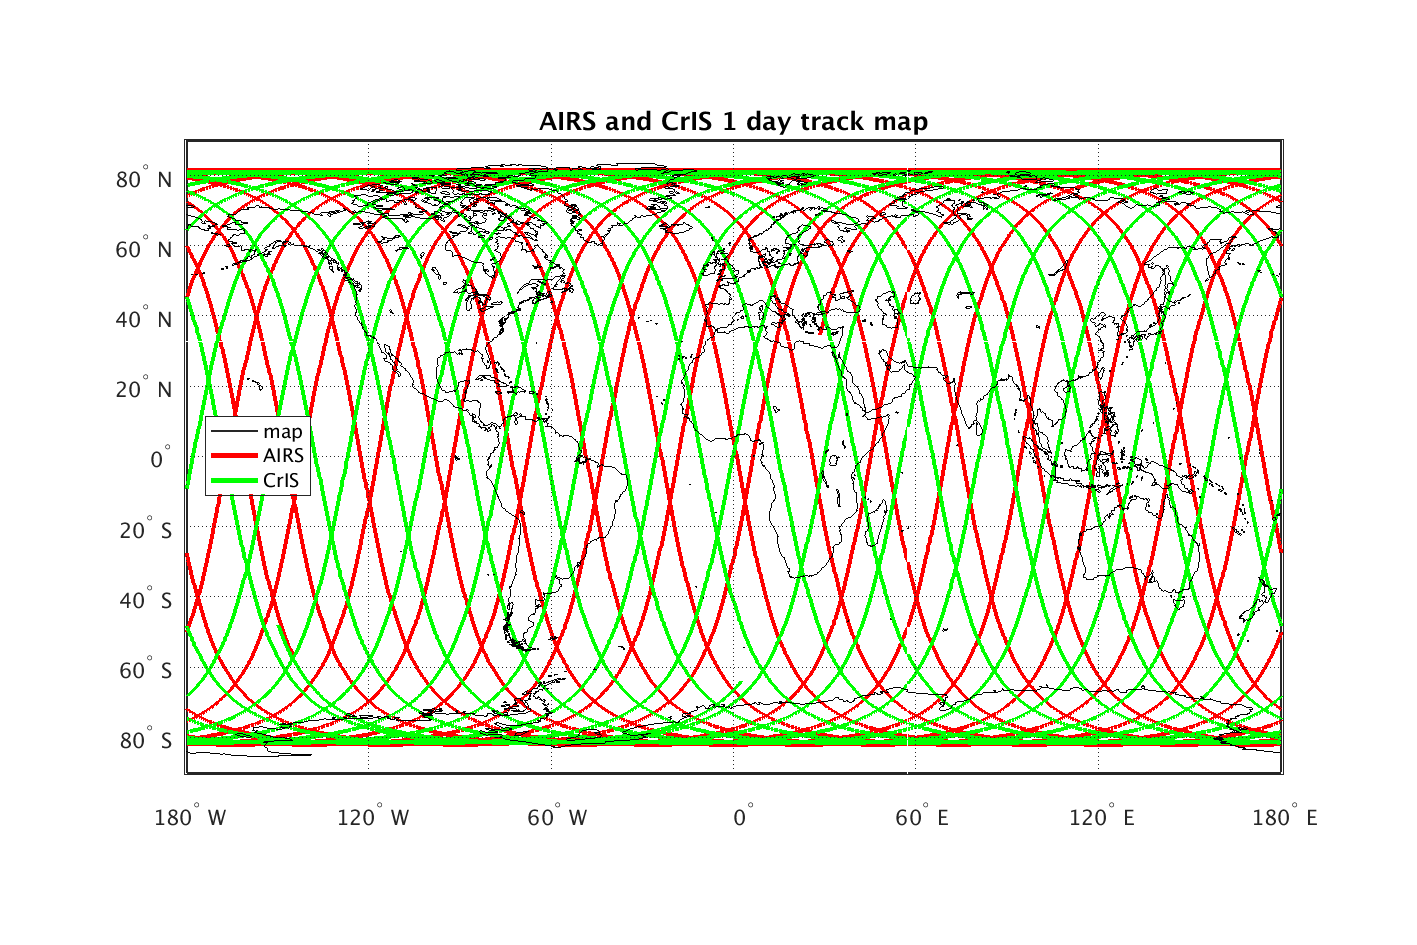
\includegraphics[scale=0.5]{figures/subpt_1_day_all.png}
\end{center}
\end{frame} % source plot_subpt.m
%----------- slide --------------------------------------------------%
\begin{frame}
\frametitle{16 day track maps}
\begin{center}
  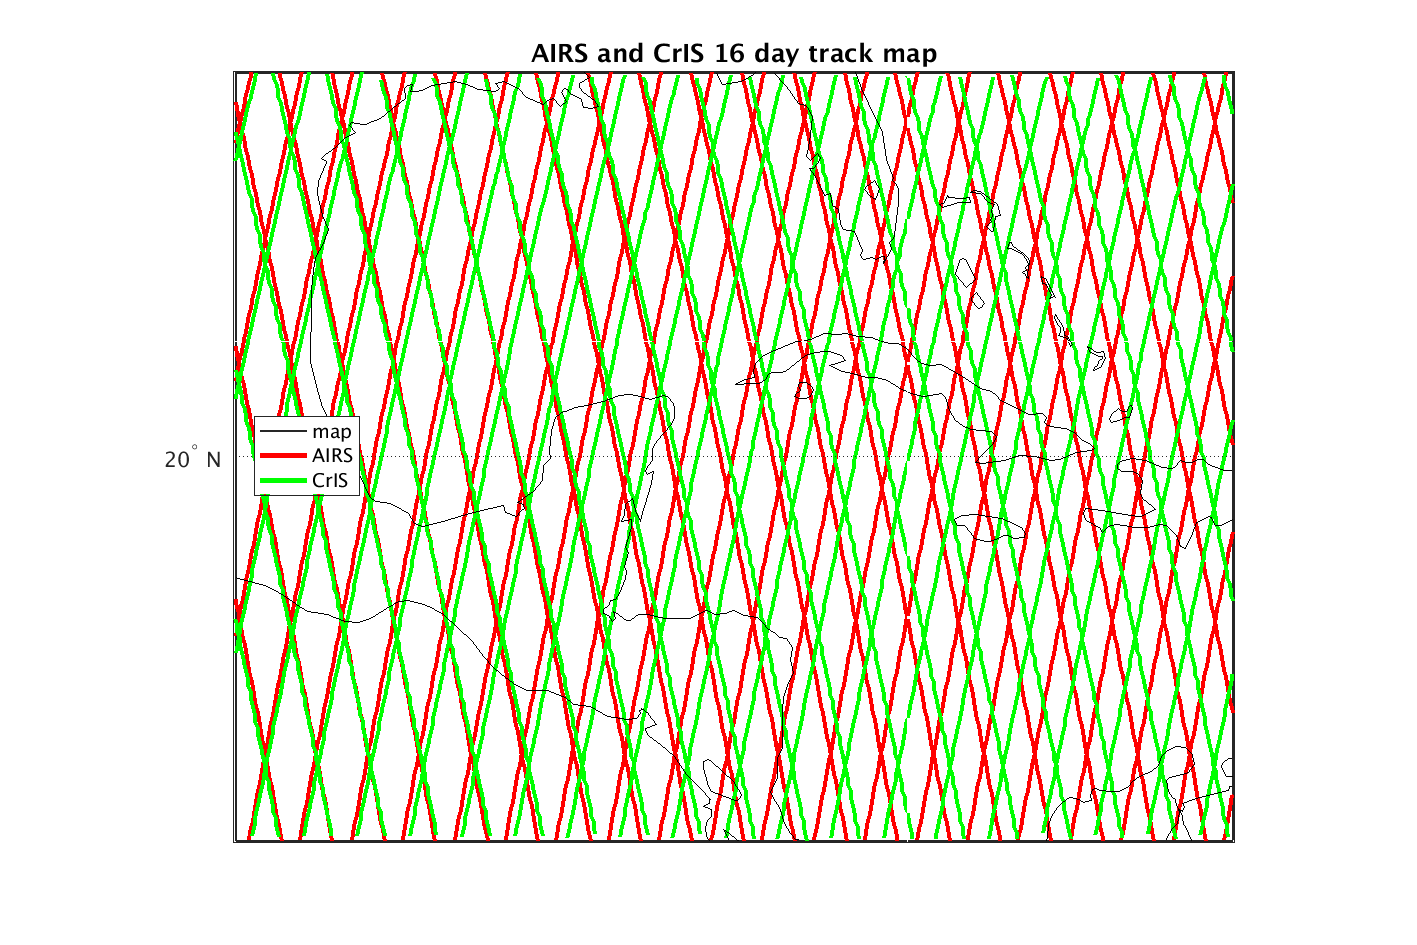
\includegraphics[scale=0.5]{figures/subpt_16_day_zoom.png}
\end{center}
\end{frame} % source plot_subpt.m
%----------- slide --------------------------------------------------%
\begin{frame}
\frametitle{AIRS and CrIS secant of zenith angles}

\begin{center}
  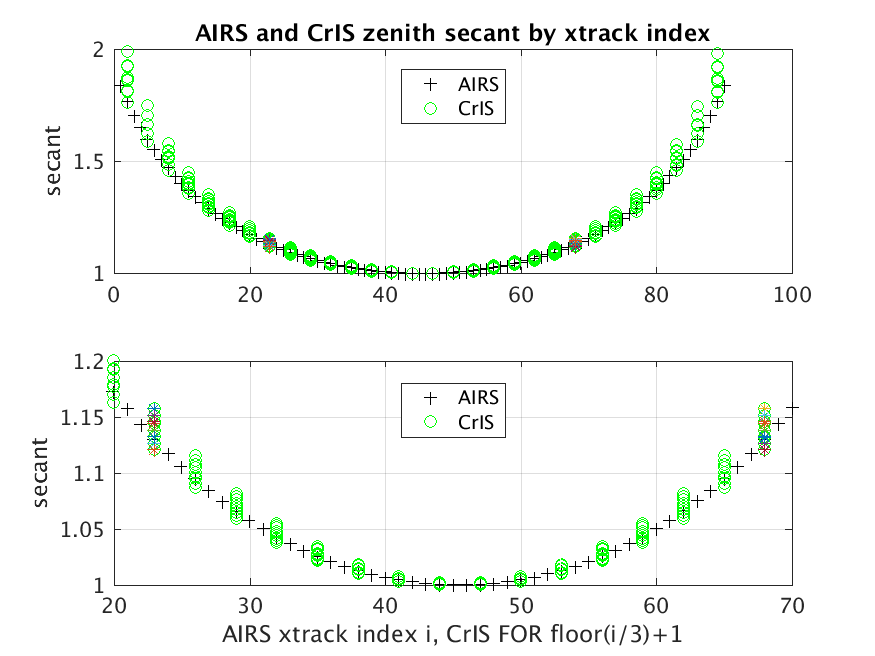
\includegraphics[scale=0.7]{figures/AIRS_CrIS_secant_by_xtrack.png}
\end{center}
\end{frame} % source plot_tbin.m
%----------- slide --------------------------------------------------%
\begin{frame}
\frametitle{test data}

\begin{itemize}

 \item most comparison tests of orbital parameters shown here are
   done with a 16 day data set from 20 Apr to 5 May 2016, chosen for
   no missing {\airs} or {\cris} obs
 
 \item PDFs are shown for the 16 day set, the 2016 seasons, and all
   of 2016 broken out by land and ocean

 \item aside from some of the final {\cris}-only FOV comparisons,
   all tests and PDFs shown here were done with both ascending and
   descending orbital phase

 \item tests shown here are with either near-nadir or full scans;
   near-nadir for {\airs} is cross-track indices 43--48, and for
   {\cris} fields of regard 15 and 16

\end{itemize}
\end{frame}
%----------- slide --------------------------------------------------%
\begin{frame}
\frametitle{equal area bands and bins}

\begin{itemize}

  \item we use latitude bands to test our latitude weighted
    subsetting, and equal area bins to examine obs and mean times
    per bin to compare {\airs} and {\cris} sampling

  \item equal area bins are formed from 24 equal area latitude bands
    from pole to equator (and so 48 bands total) and longitude steps
    of 4 degrees

  \item we have looked at other binning parameters; smaller bins
    give greater variation.  The values chosen may be reasonable for
    evaulating samping for long span tests

  \item the equal area subsetting is not actually used in the
    tabulation of PDFs; the bins there are brightness temperature
    obs counts

\end{itemize}
\end{frame}
%----------- slide --------------------------------------------------%
\begin{frame}
\frametitle{CrIS 16--day near-nadir obs count by latitude band}
\begin{center}
  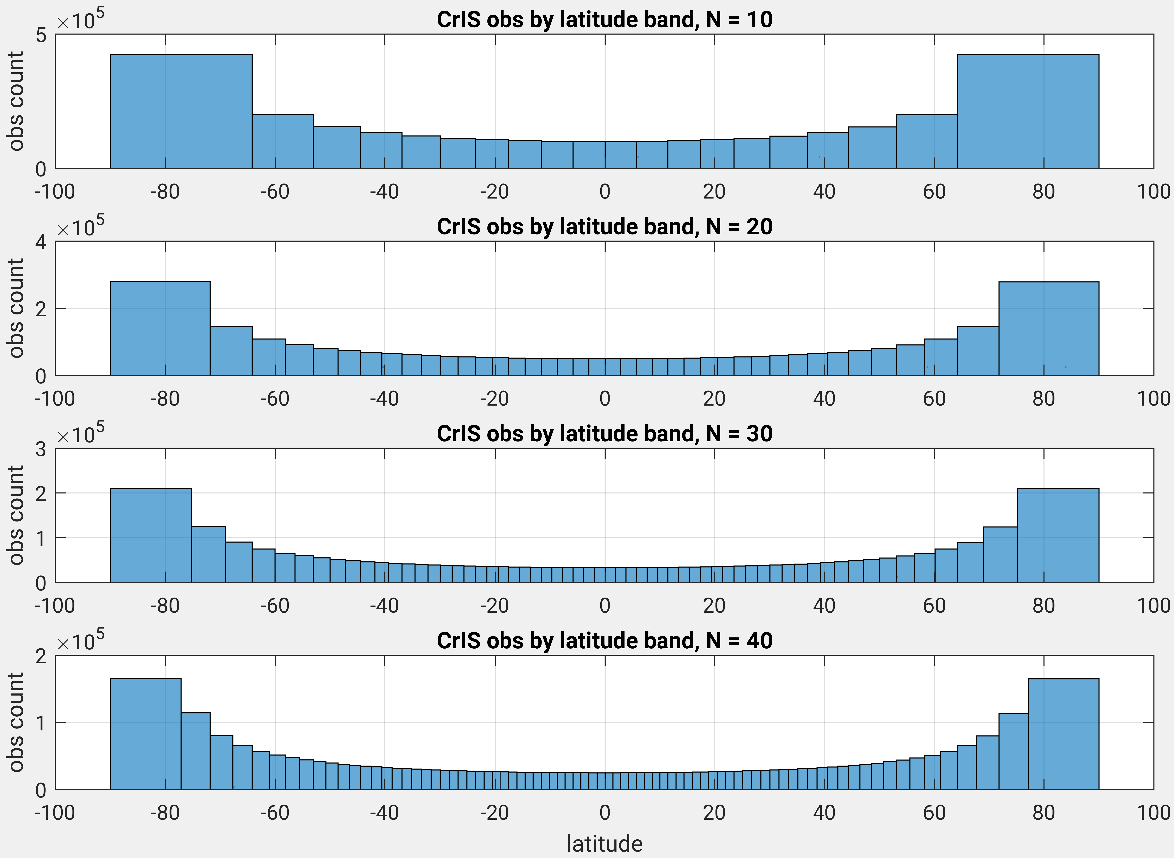
\includegraphics[scale=0.5]{figures/cris_obs_by_lat_band.pdf}
\end{center}
\end{frame} % source cris_obslist.m
%----------- slide --------------------------------------------------%
\begin{frame}
\frametitle{latitude weighted subsetting}

\begin{itemize}

  \item we want to do global stats with equal area sampling

  \item {\airs} and {\cris} oversample significantly towards the
    poles, so we want to drop some of those obs

  \item a simple heuristic is to keep all obs such that $X <
    \abs(\cos(\lat))$, where $X$ is a random variable from the
    uniform distribution $[0, 1]$

  \item as shown on subsequent slides, this works fairly well. \\ It
    is not hard to do better; for example $X <
    \abs(\cos(\lat)^{1.1})$ gives more uniform sampling for $N$ up
    to around 40.  But that is a hack.

  \item all subsequent results here, and in particular all the PDFs,
    are done with the basic cosine subsetting unless otherwise noted

\end{itemize}
\end{frame}
%----------- slide --------------------------------------------------%
\begin{frame}
\frametitle{CrIS cosine of latitude subset}
\begin{center}
  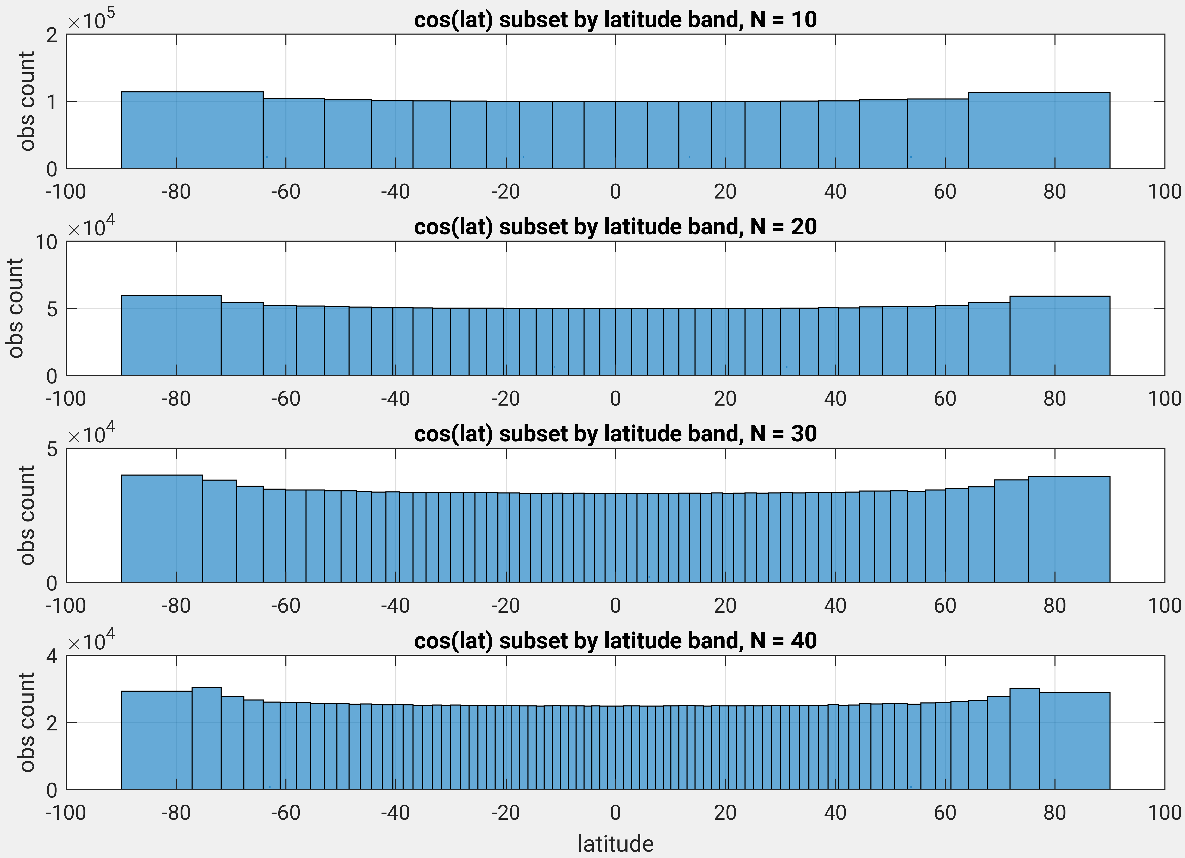
\includegraphics[scale=0.5]{figures/cris_cos_lat_subset.pdf}
\end{center}
\end{frame} % source cris_obslist.m
%----------- slide --------------------------------------------------%
\begin{frame}
\frametitle{AIRS cosine of latitude subset}
\begin{center}
  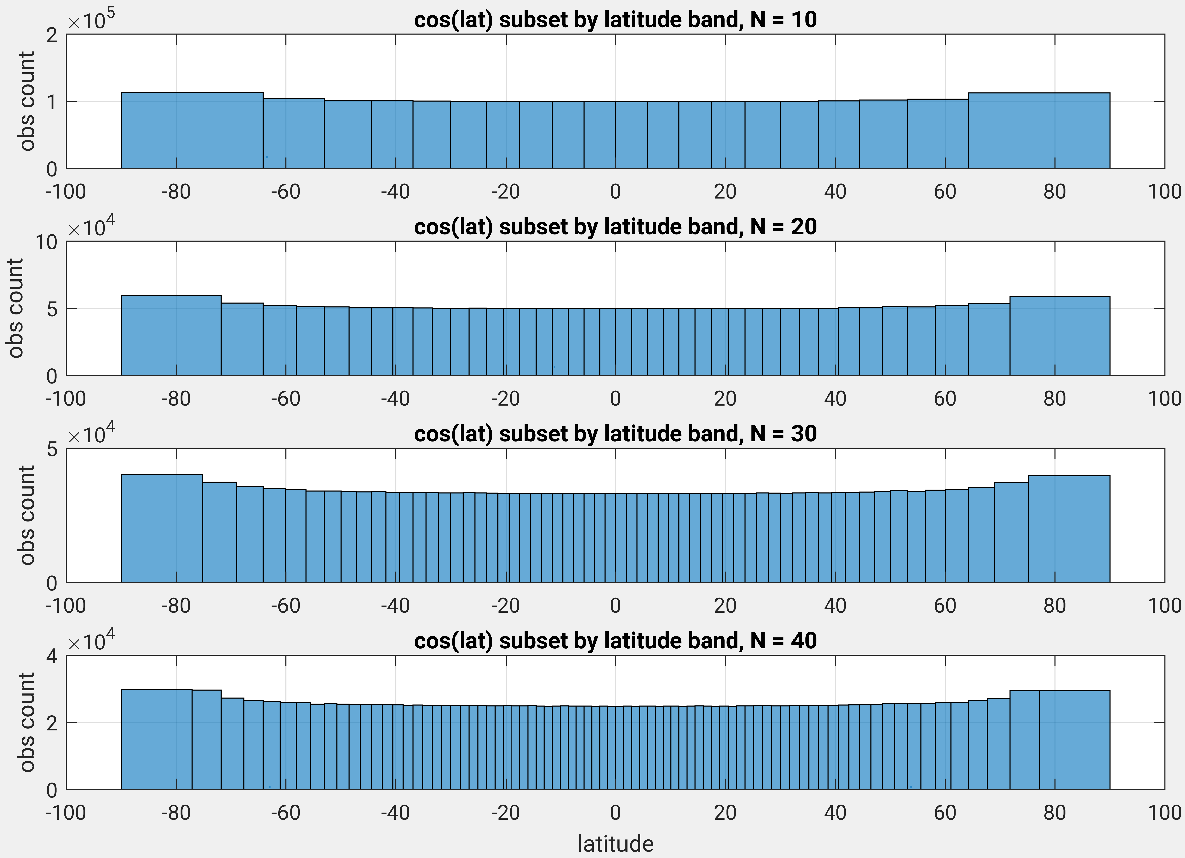
\includegraphics[scale=0.5]{figures/airs_cos_lat_subset.pdf}
\end{center}
\end{frame} % source airs_obslist.m
%----------- slide --------------------------------------------------%
\begin{frame}
\frametitle{AIRS and CrIS sampling comparisons}

\begin{itemize}

  \item we compare obs counts and time differences per equal area
    bin for AIRS and CrIS near-nadir and full scan obs

  \item Let $c_i$ be the obs count for bin $i$, and $m$ the mean of
    $c_i$ over all bins for a particular instrument and test.  Then
    $(c_i - m) / m$ is the relative count for bin $i$.  This is what
    we show for the single-instrument maps.  We also consider the
    difference of two such maps

  \item similarly, let $t_i$ be the mean obs time for bin $i$ and
    $n$ the mean time over all obs in the test; then $t_i - n$ is
    the time difference for bin $i$.  This is what we show for the
    single-instrument maps.  As with relative obs counts, we also
    consider the difference of two such maps.   In both cases the
    units for the colormaps are days.

\end{itemize}
\end{frame}
%----------- slide --------------------------------------------------%
\begin{frame}
\frametitle{CrIS near-nadir relative obs count by equal area bin}
\begin{center}
  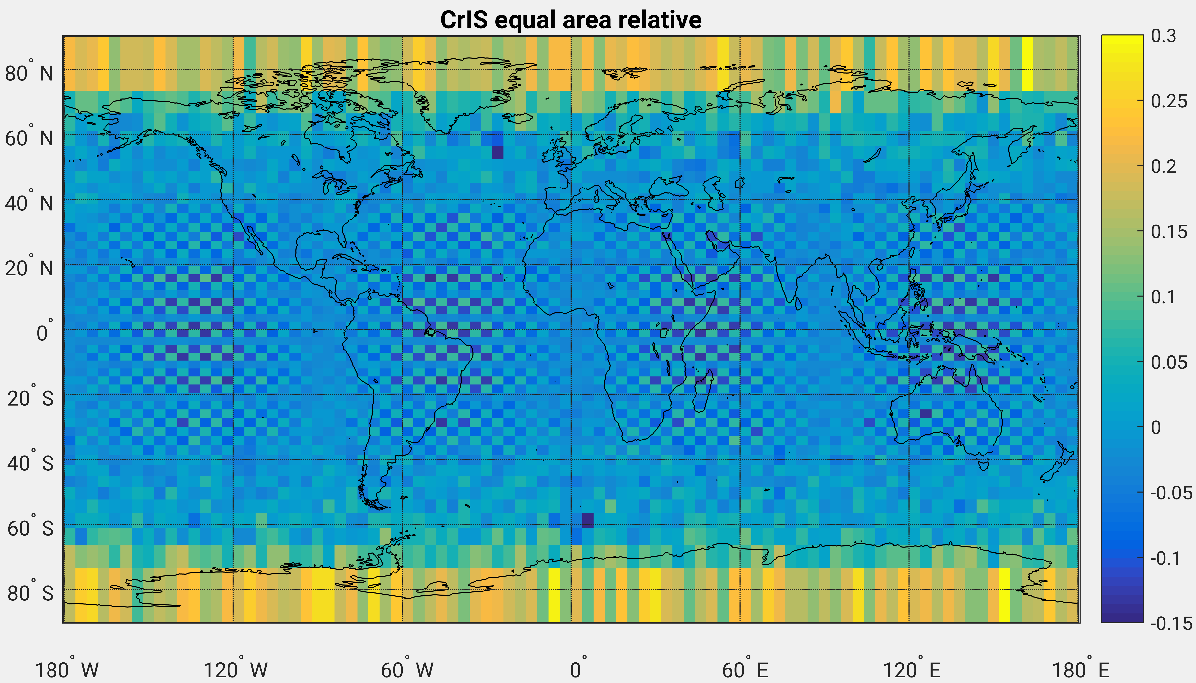
\includegraphics[scale=0.5]{figures/cris_eq_area_rel_obs_d1s1w1.pdf}
\end{center}
\end{frame} % source plot_obsbin.m
%----------- slide --------------------------------------------------%
\begin{frame}
\frametitle{AIRS near-nadir relative obs count by equal area bin}
\begin{center}
  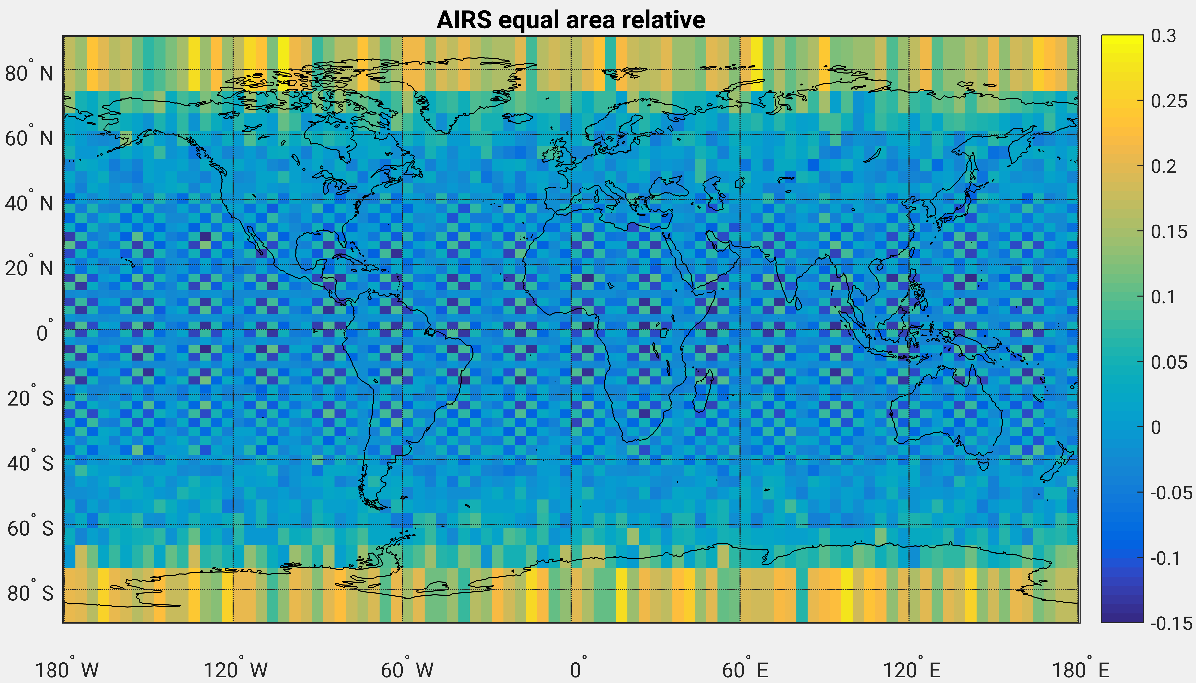
\includegraphics[scale=0.5]{figures/airs_eq_area_rel_obs_d1s1w1.pdf}
\end{center}
\end{frame} % source plot_obsbin.m 
%----------- slide --------------------------------------------------%
\begin{frame}
\frametitle{CrIS minus AIRS near-nadir relative obs difference}
\begin{center}
  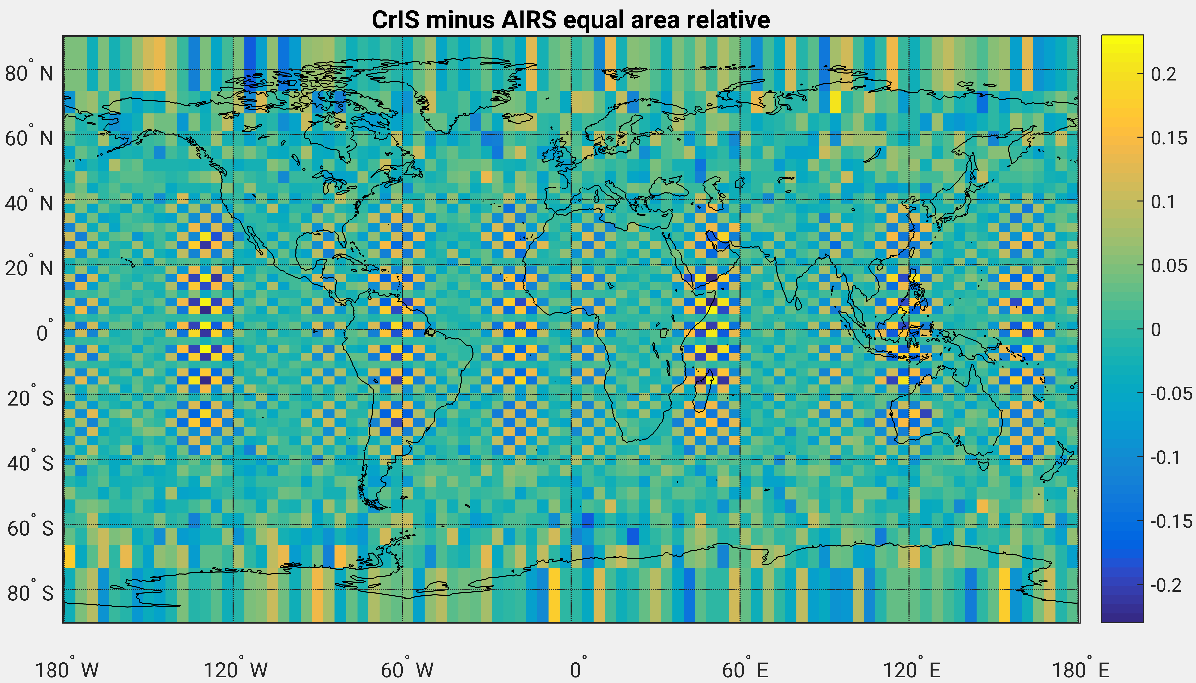
\includegraphics[scale=0.5]{figures/cris_minus_airs_obs_d1s1w1.pdf}
\end{center}
\end{frame} % source plot_obsbin.m
%----------- slide --------------------------------------------------%
\begin{frame}
\frametitle{CrIS minus AIRS full-scan relative obs difference}
\begin{center}
  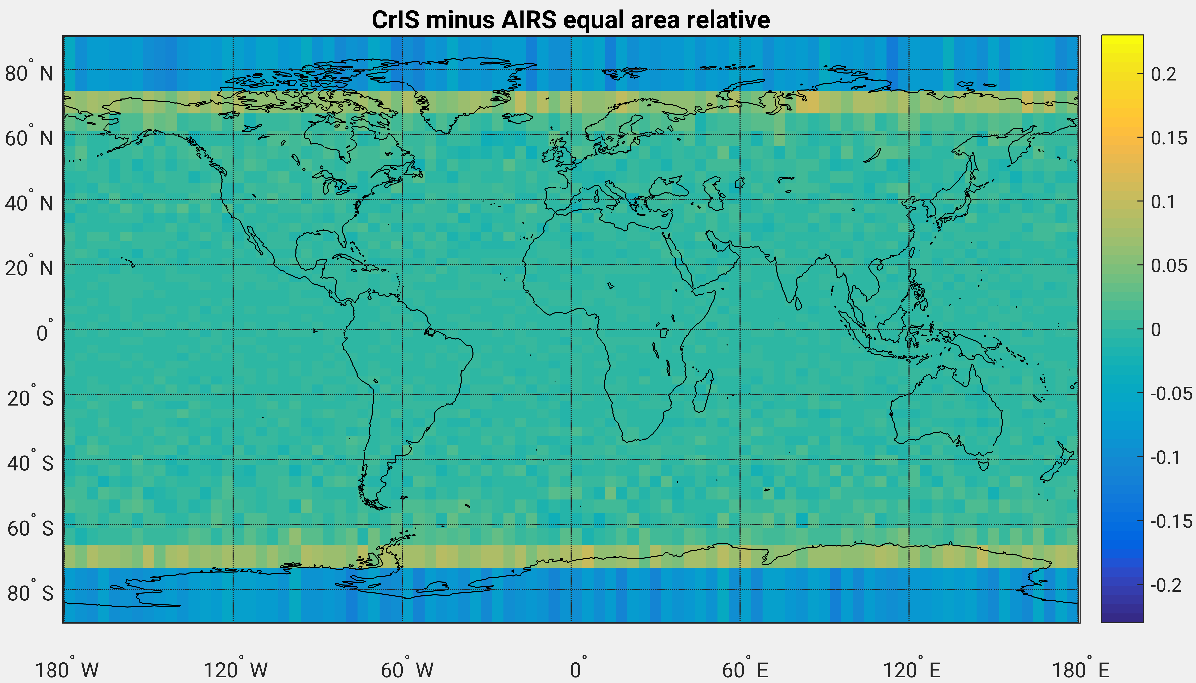
\includegraphics[scale=0.5]{figures/cris_minus_airs_obs_d1s2w1.pdf}
\end{center}
\end{frame} % source plot_obsbin.m
%----------- slide --------------------------------------------------%
\begin{frame}
\frametitle{CrIS near-nadir mean time by equal area bin}
\begin{center}
  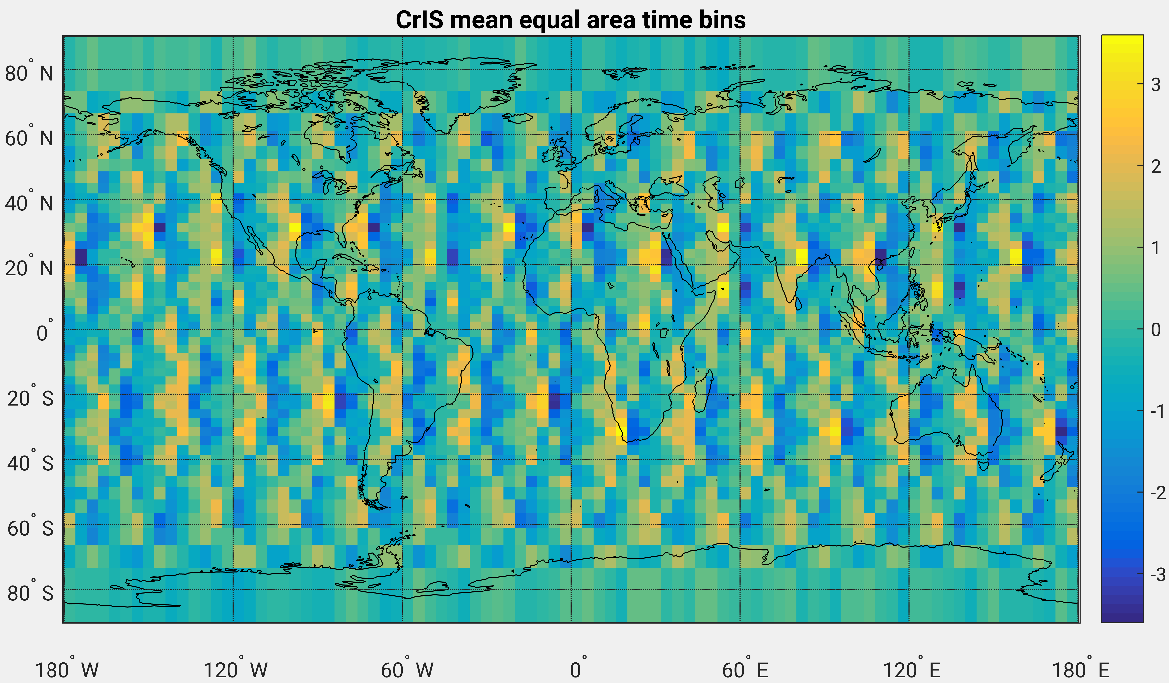
\includegraphics[scale=0.5]{figures/cris_eq_area_rel_time_d1s1w1.pdf}
\end{center}
\end{frame} % source plot_timebin.m
%----------- slide --------------------------------------------------%
\begin{frame}
\frametitle{AIRS near-nadir mean time by equal area bin}
\begin{center}
  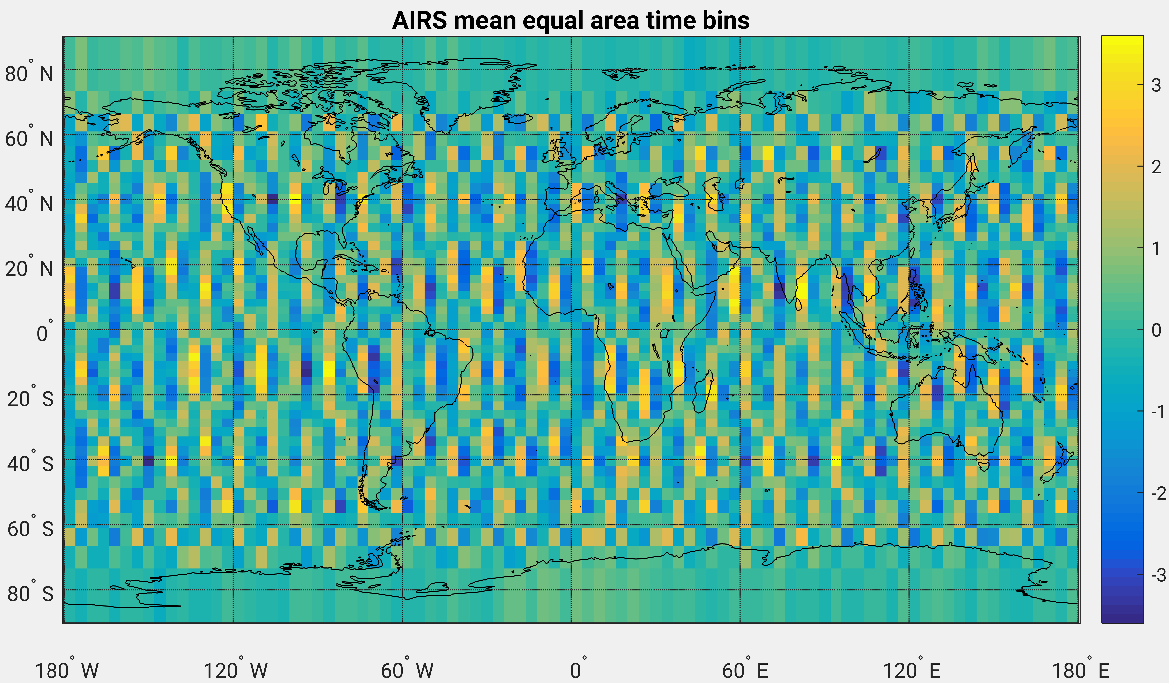
\includegraphics[scale=0.5]{figures/airs_eq_area_rel_time_d1s1w1.pdf}
\end{center}
\end{frame} % source plot_timebin.m 
%----------- slide --------------------------------------------------%
\begin{frame}
\frametitle{CrIS minus AIRS near-nadir time difference}
\begin{center}
  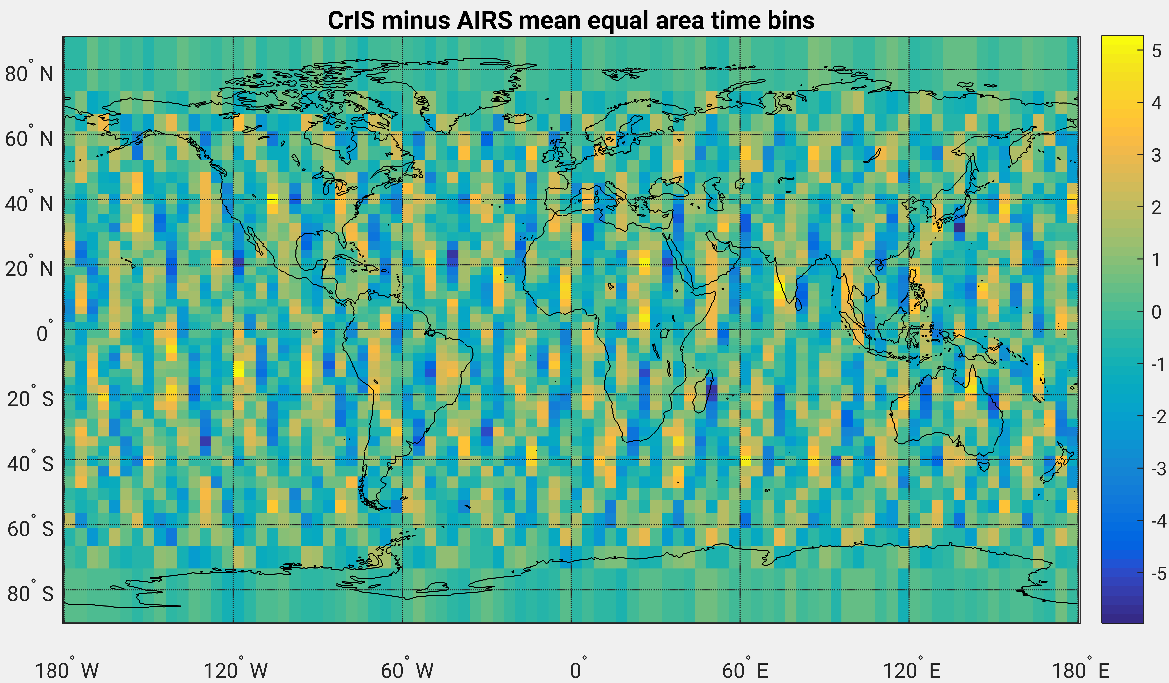
\includegraphics[scale=0.5]{figures/cris_minus_airs_time_d1s1w1.pdf}
\end{center}
\end{frame} % source plot_timebin.m
%----------- slide --------------------------------------------------%
\begin{frame}
\frametitle{CrIS minus AIRS full-scan time difference}
\begin{center}
  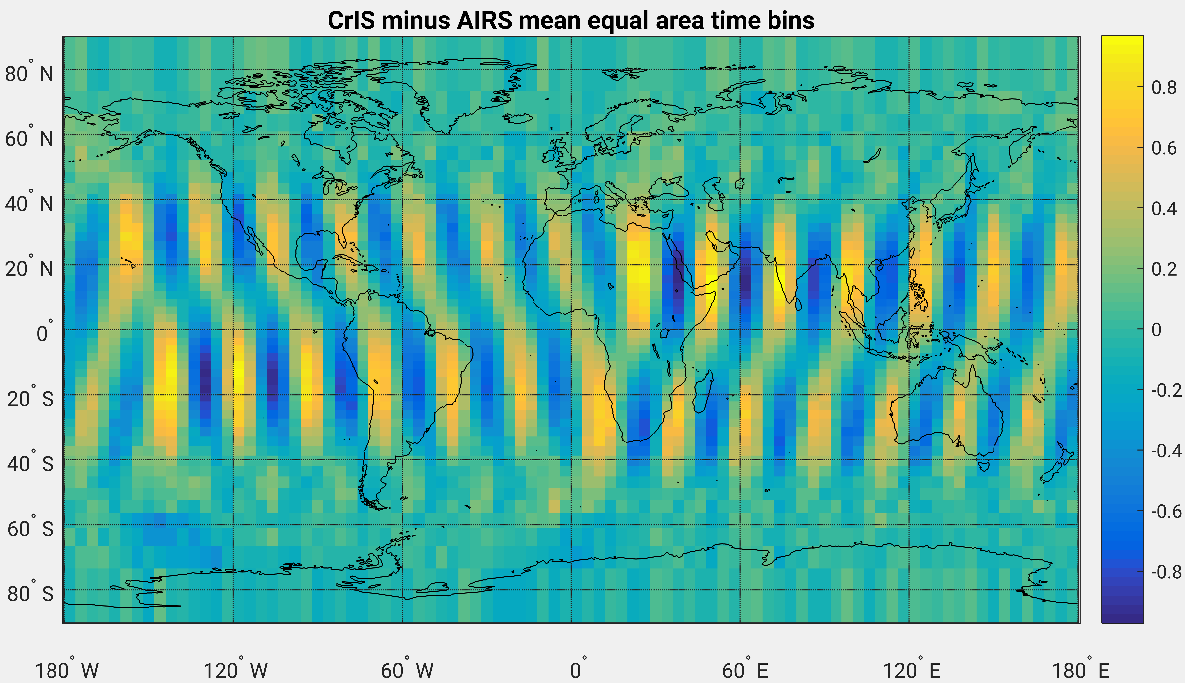
\includegraphics[scale=0.5]{figures/cris_minus_airs_time_d1s2w1.pdf}
\end{center}
\end{frame} % source plot_timebin.m
%----------- slide --------------------------------------------------%
\begin{frame}
\frametitle{AIRS and CrIS PDFs}
\begin{itemize}

  \item we create PDFs (or obs per $T_b$ bin tabulations) for
    {\airs} and {\cris} as follows

\begin{enumerate}
  \item choose a test period and any subsetting options

  \item tabulate obs by $T_b$ bin the test periods, for both {\airs}
    and {\cris}.  Let $n_a$ be the total number of {\airs} and $n_c$
    the total number of {\cris} obs.  Continue only if $n_a$ and
    $n_c$ are close, typically within about 1 pct

  \item normalize the {\cris} counts to {\airs}, multiplying by
    $n_a/n_c$.

  \item examine the relative difference of the normalized counts.  \\
    If $k_a$ and $k_c$ are {\airs} and {\cris} counts for $T_b$ bin
    $K$, this is $( k_c n_a/n_c - k_a) / k_a$.
\end{enumerate}

  \item to increase the sample space, we would like to work with
    full scans, if possible

\end{itemize}
\end{frame}
%----------- slide --------------------------------------------------%
\begin{frame}
\frametitle{16 day near-nadir obs by Tb bin}
\begin{center}
  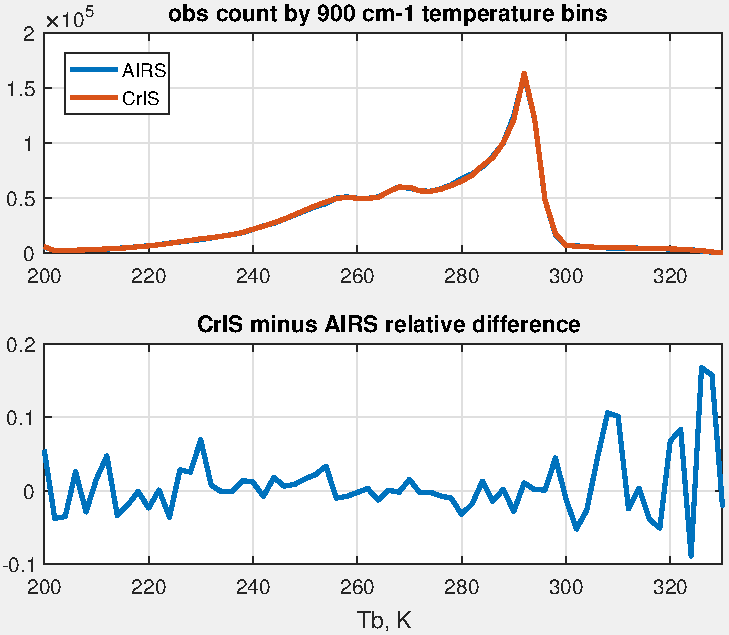
\includegraphics[scale=0.7]{figures/plot_tbin_test_11.pdf}
\end{center}
\end{frame} % source plot_tbin.m
%----------- slide --------------------------------------------------%
\begin{frame}
\frametitle{16 day full scan obs by Tb bin}
\begin{center}
  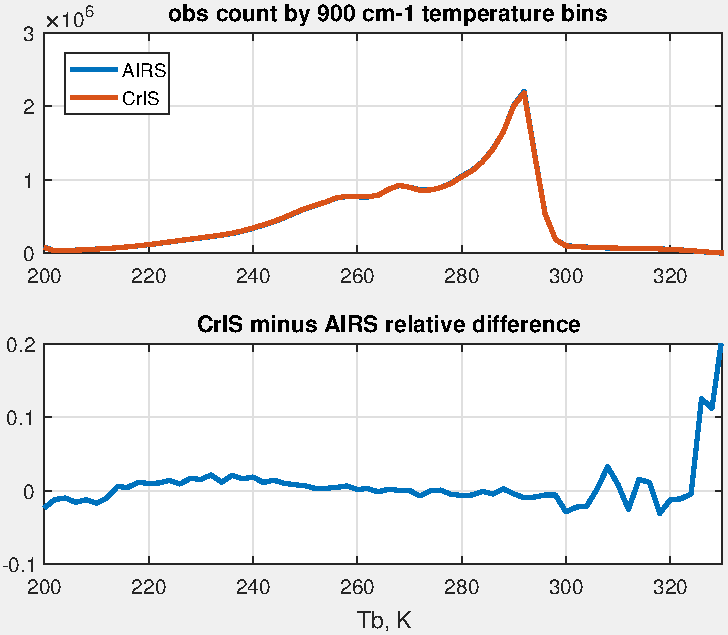
\includegraphics[scale=0.7]{figures/plot_tbin_test_31.pdf}
\end{center}
\end{frame} % source plot_tbin.m
%----------- slide --------------------------------------------------%
\begin{frame}
\frametitle{2016 winter full-scan land only}
\begin{center}
  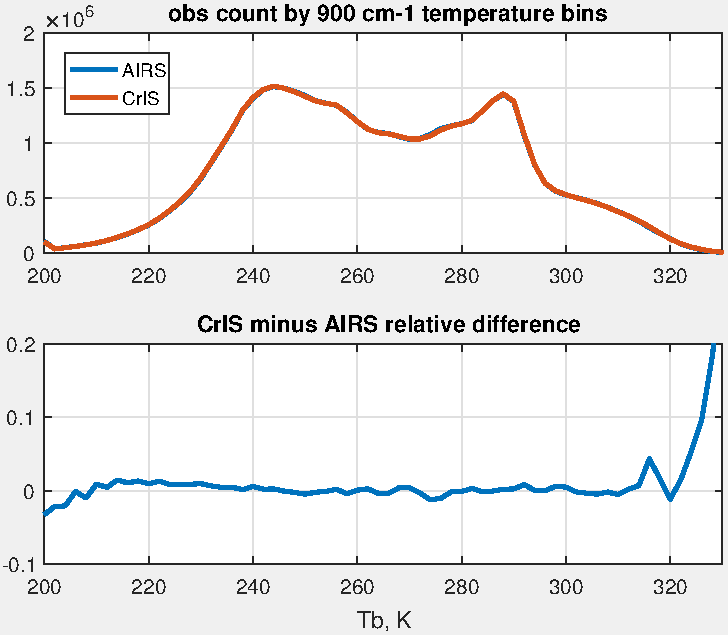
\includegraphics[scale=0.7]{figures/full-scan_land_2016_winter.pdf}
\end{center}
\end{frame} % source plot_tbin.m
%----------- slide --------------------------------------------------%
\begin{frame}
\frametitle{2016 spring full scan land only}
\begin{center}
  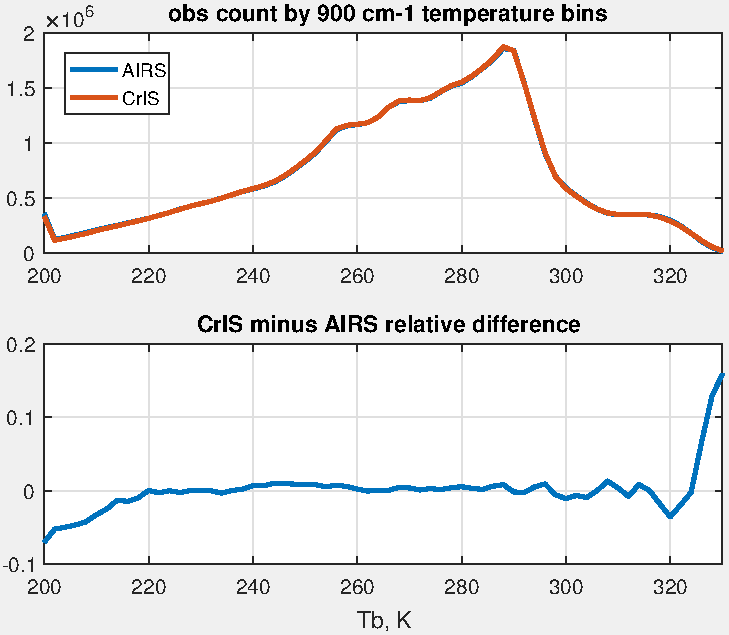
\includegraphics[scale=0.7]{figures/full-scan_land_2016_spring.pdf}
\end{center}
\end{frame} % source plot_tbin.m
%----------- slide --------------------------------------------------%
\begin{frame}
\frametitle{2016 summer full scan land}
\begin{center}
  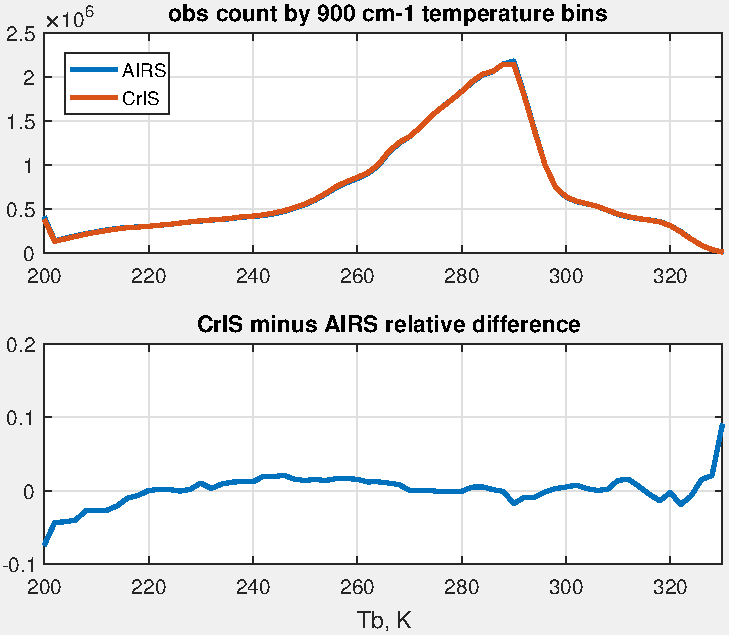
\includegraphics[scale=0.7]{figures/full-scan_land_2016_summer.pdf}
\end{center}
\end{frame} % source plot_tbin.m
%----------- slide --------------------------------------------------%
\begin{frame}
\frametitle{2016 fall full scan land}
\begin{center}
  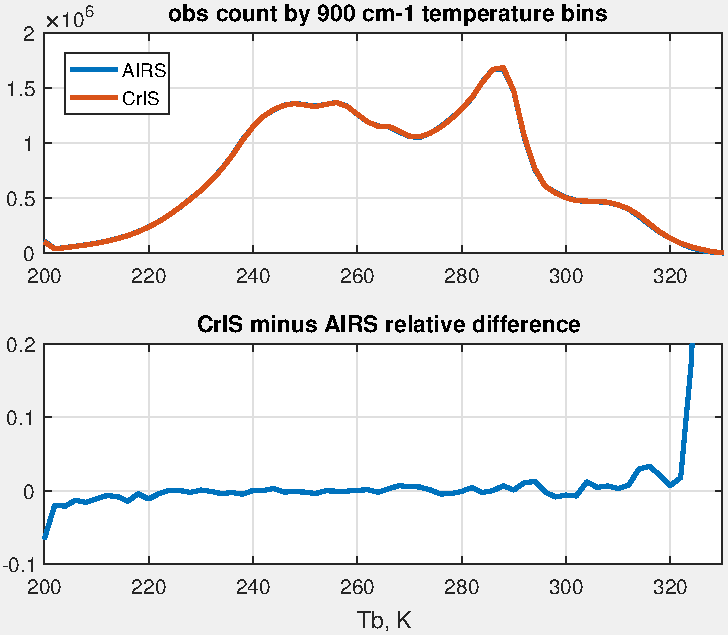
\includegraphics[scale=0.7]{figures/full-scan_land_2016_fall.pdf}
\end{center}
\end{frame} % source plot_tbin.m
%----------- slide --------------------------------------------------%
\begin{frame}
\frametitle{2016 full year full scan land}
\begin{center}
  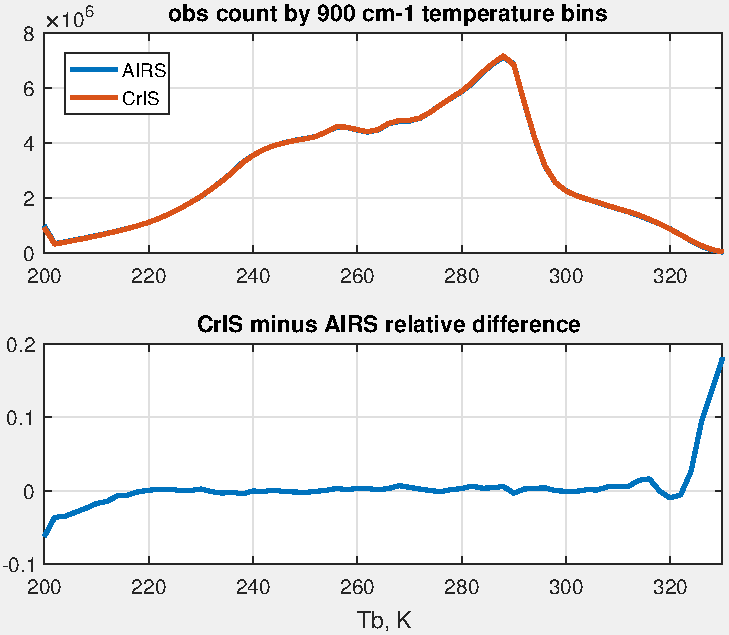
\includegraphics[scale=0.7]{figures/full-scan_land_2016_all.pdf}
\end{center}
\end{frame} % source plot_tbin.m
%----------- slide --------------------------------------------------%
\begin{frame}
\frametitle{2016 full year full scan ocean}
\begin{center}
  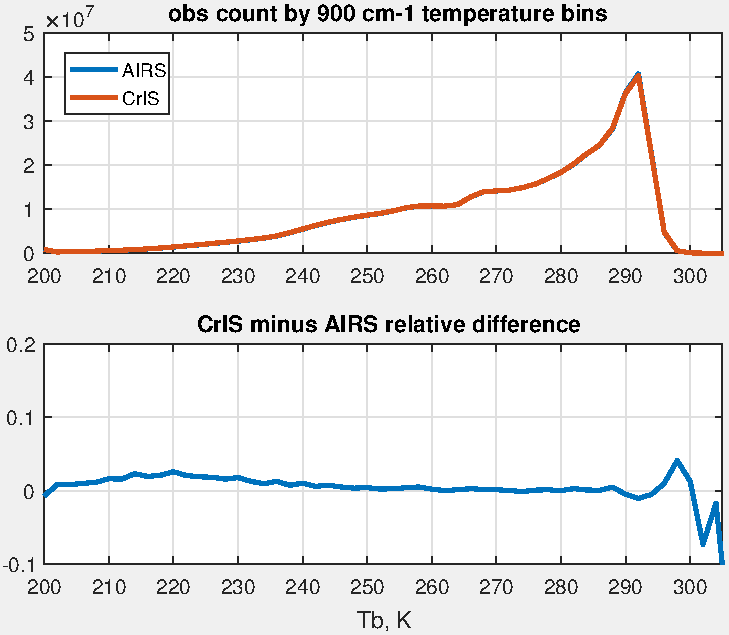
\includegraphics[scale=0.7]{figures/full-scan_ocean_2016_all.pdf}
\end{center}
\end{frame} % source plot_tbin.m
%----------- slide --------------------------------------------------%
\begin{frame}
\frametitle{CrIS FOV comparisons}

\begin{itemize}

  \item in these tests we apply our methods for {\airs} and {\cris}
    comparisons to individual {\cris} {\fov}s

  \item the range of test parameters is expanded; we look at both
    ascending and descending together and descending alone, and
    binning at both coarser and finer resolutions

  \item the next group of tests is from the 20 April 2016 16 day
    set, near-nadir only (FOR 15 and 16), with latitude weighted
    subsetting turned on.   

  \item the time differences are calculated as before, but the
    72-band obs count stats are for raw obs count, not relative
    counts 

\end{itemize}

\end{frame}
%----------- slide --------------------------------------------------%
\begin{frame}
\frametitle{FOV 1 only ascending and descending}
\begin{center}
  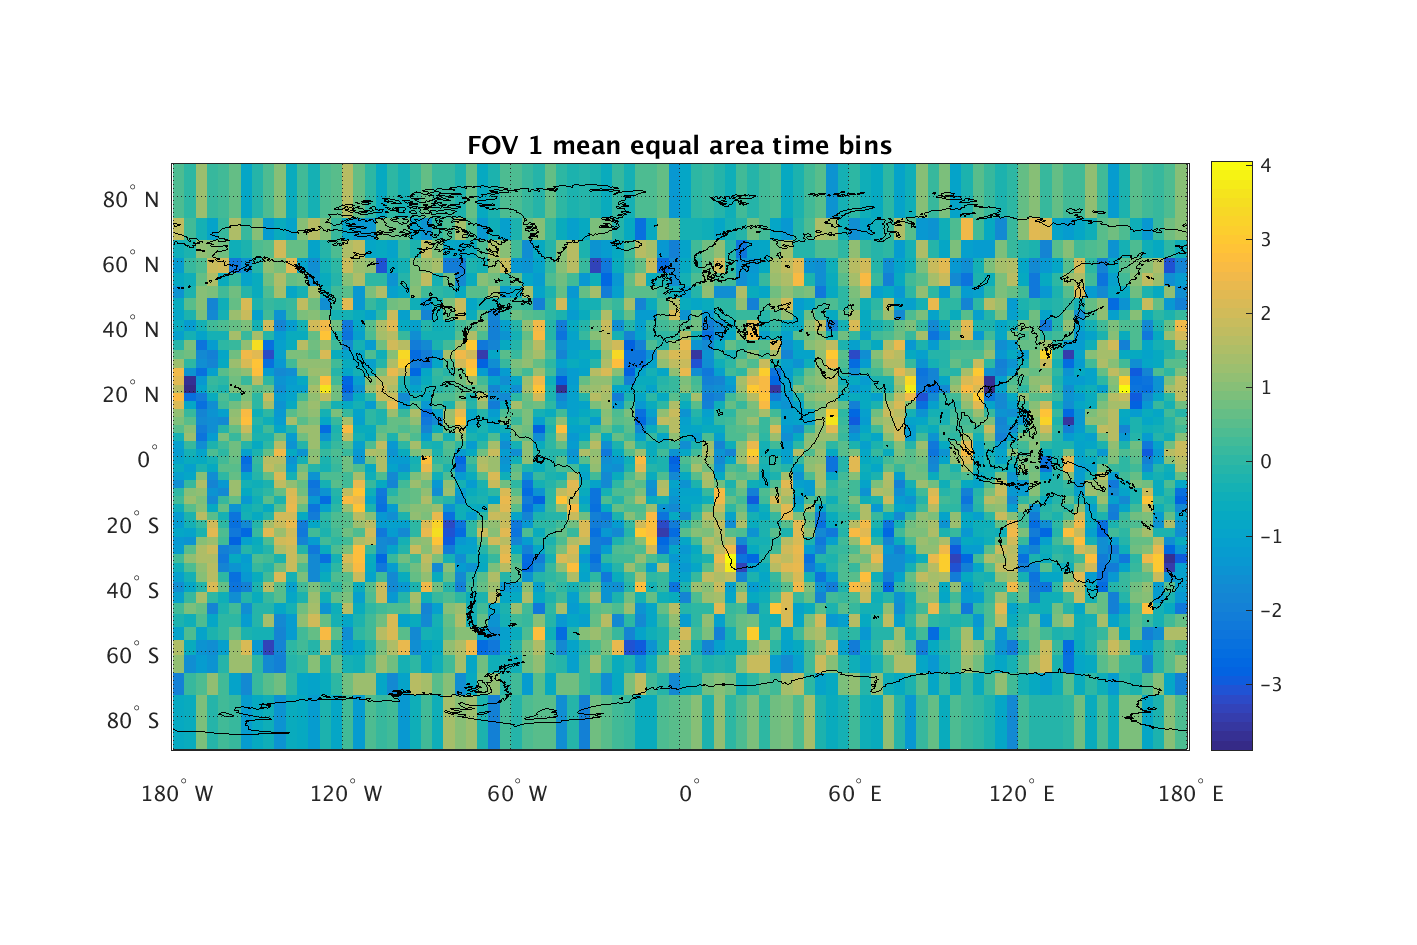
\includegraphics[scale=0.5]{slackfigs/near_nadir_FOv_1_only.png}
\end{center}
\end{frame} % slack/combined sensors 13 July 2017
%----------- slide --------------------------------------------------%
\begin{frame}
\frametitle{FOV 9 minus FOV 1 ascending and descending}
\begin{center}
  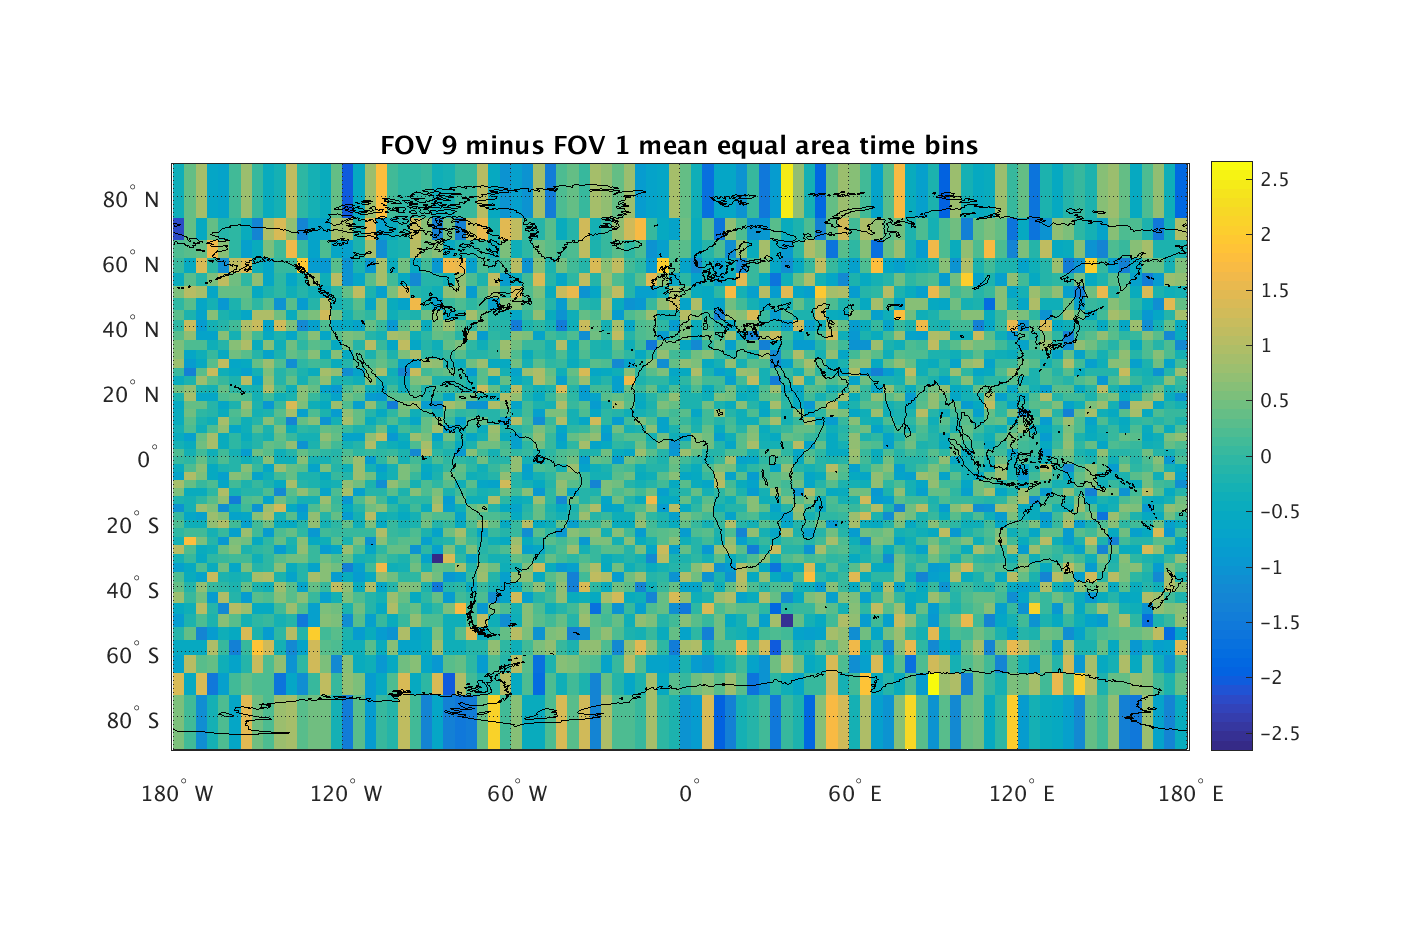
\includegraphics[scale=0.5]{slackfigs/near_nadir_FOv_1_minus_9.png}
\end{center}
\end{frame} % slack/combined sensors 13 July 2017
%----------- slide --------------------------------------------------%
\begin{frame}
\frametitle{FOV 1 descending 48 band}
\begin{center}
  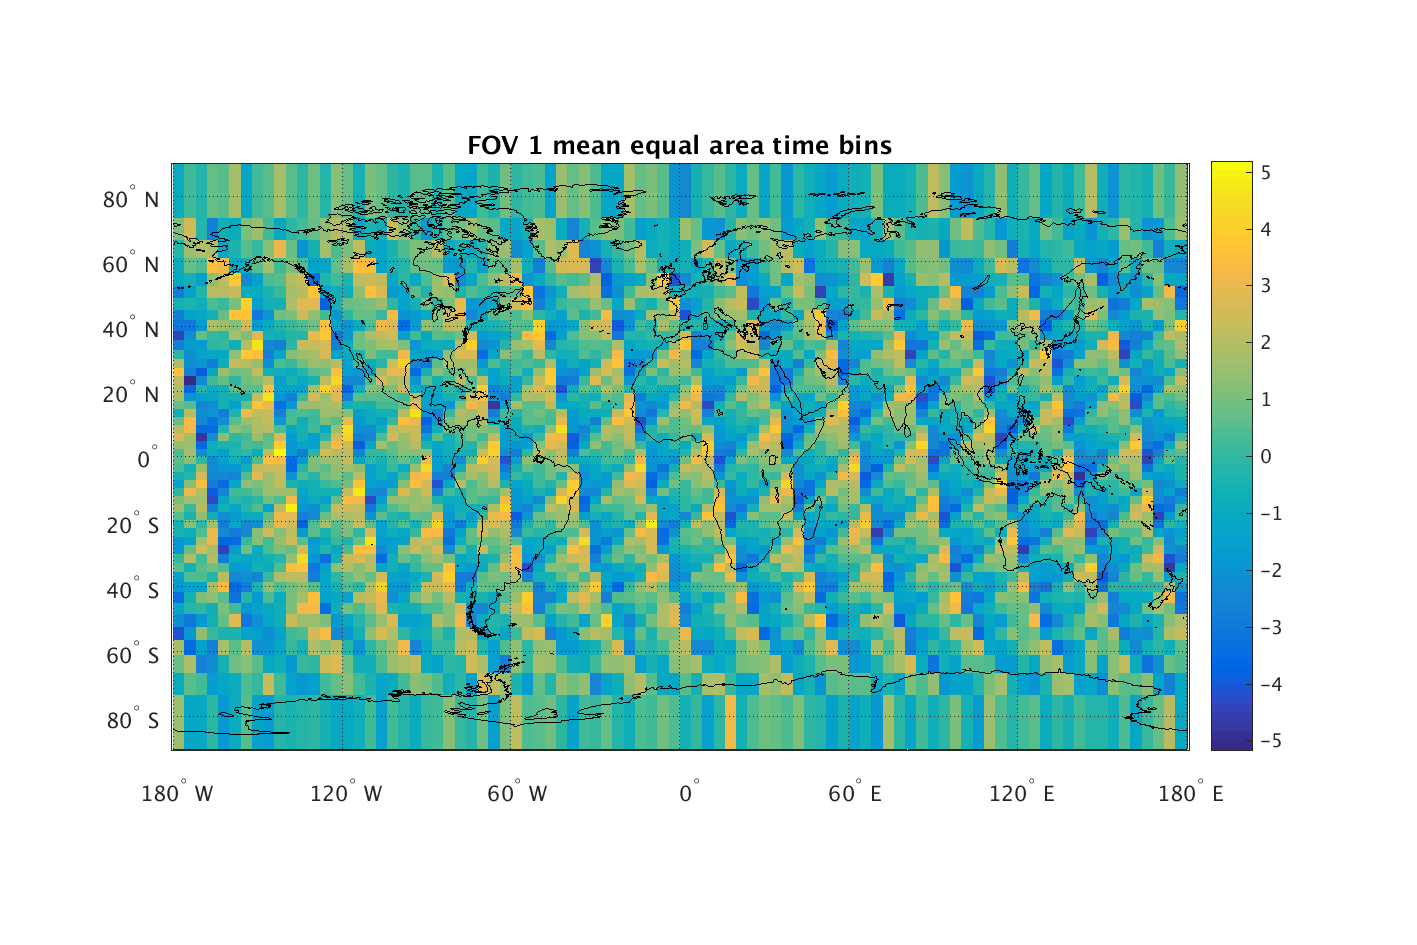
\includegraphics[scale=0.5]{slackfigs/FOV_1_48_bin_desc.png}
\end{center}
\end{frame} % slack/combined sensors 14 July 2017
%----------- slide --------------------------------------------------%
\begin{frame}
\frametitle{FOV 1 descending 40 band}
\begin{center}
  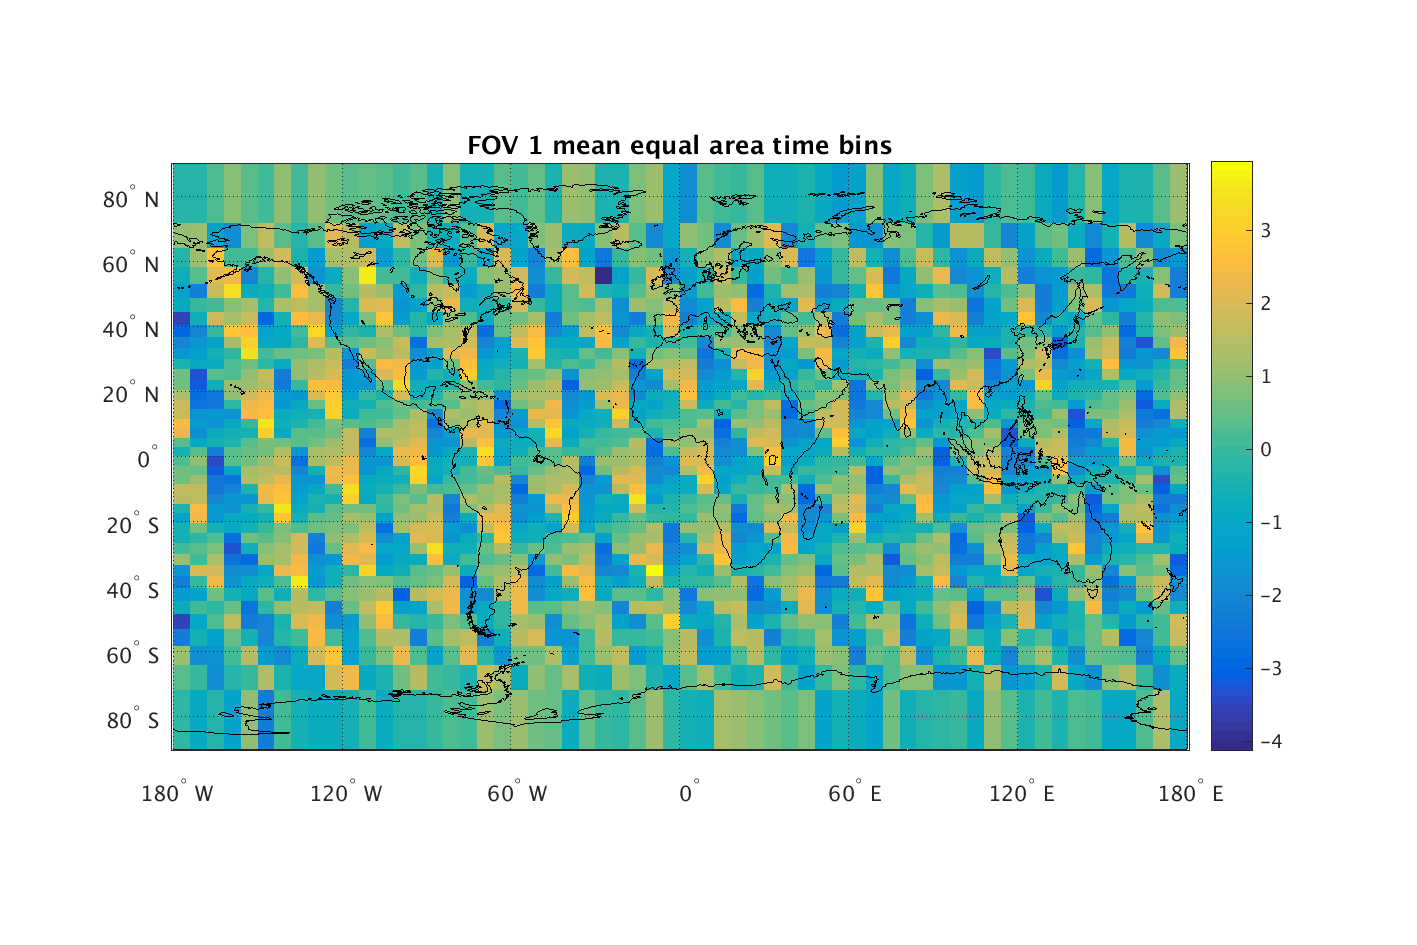
\includegraphics[scale=0.5]{slackfigs/FOV_1_40_bin_desc.png}
\end{center}
\end{frame} % slack/combined sensors 14 July 2017
%----------- slide --------------------------------------------------%
\begin{frame}
\frametitle{FOV 9 minus FOV 1 descending 40 band}
\begin{center}
  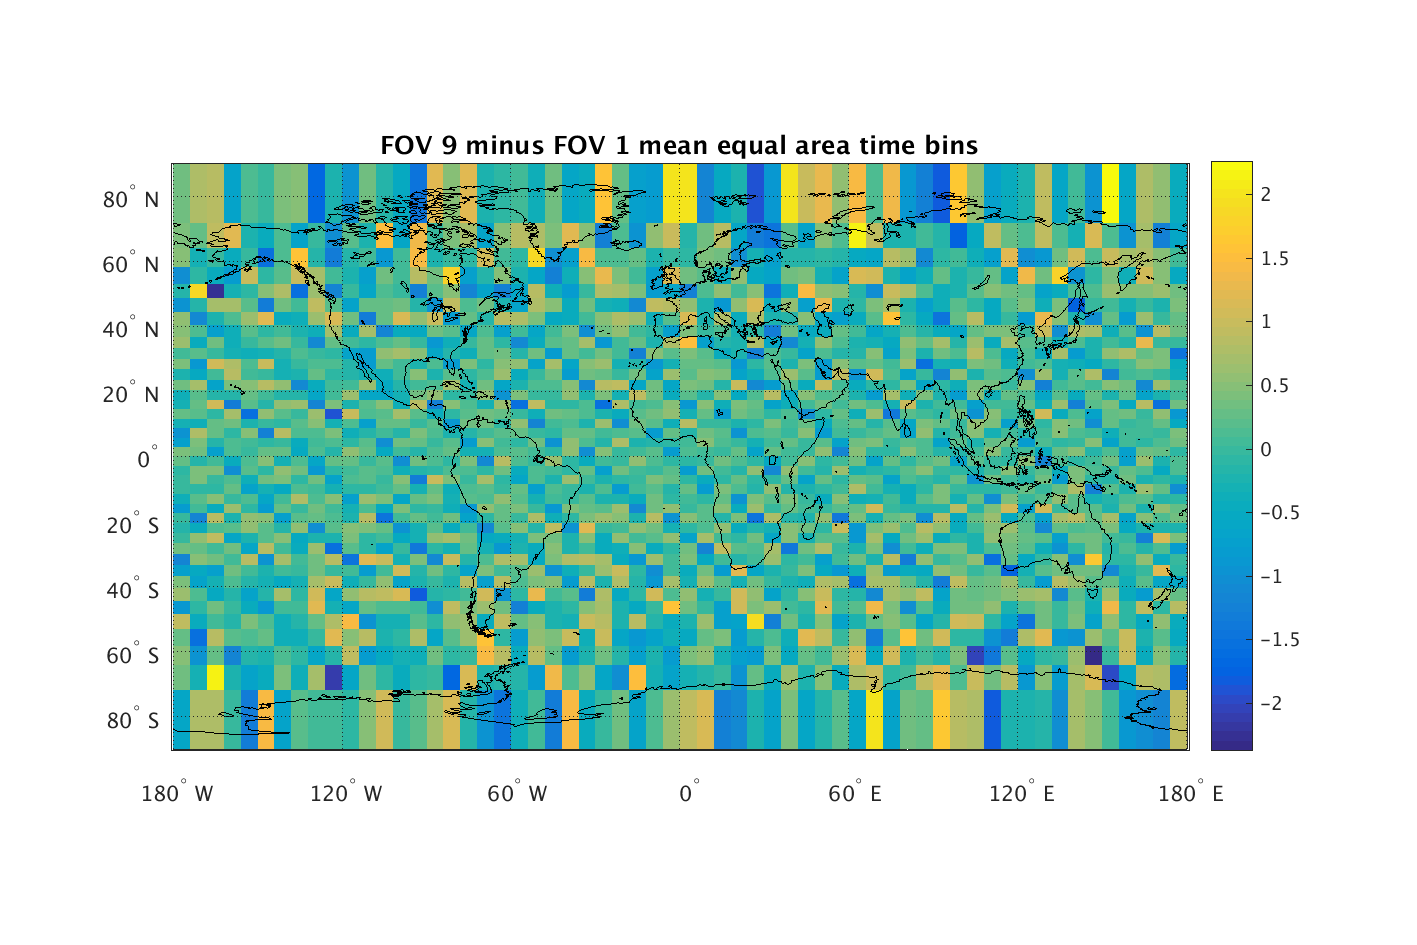
\includegraphics[scale=0.5]{slackfigs/FOV_9_minus_1_40_bin_desc.png}
\end{center}
\end{frame} % slack/combined sensors 14 July 2017
%----------- slide --------------------------------------------------%
\begin{frame}
\frametitle{FOV 1 72 band raw obs counts, descending}
\begin{center}
  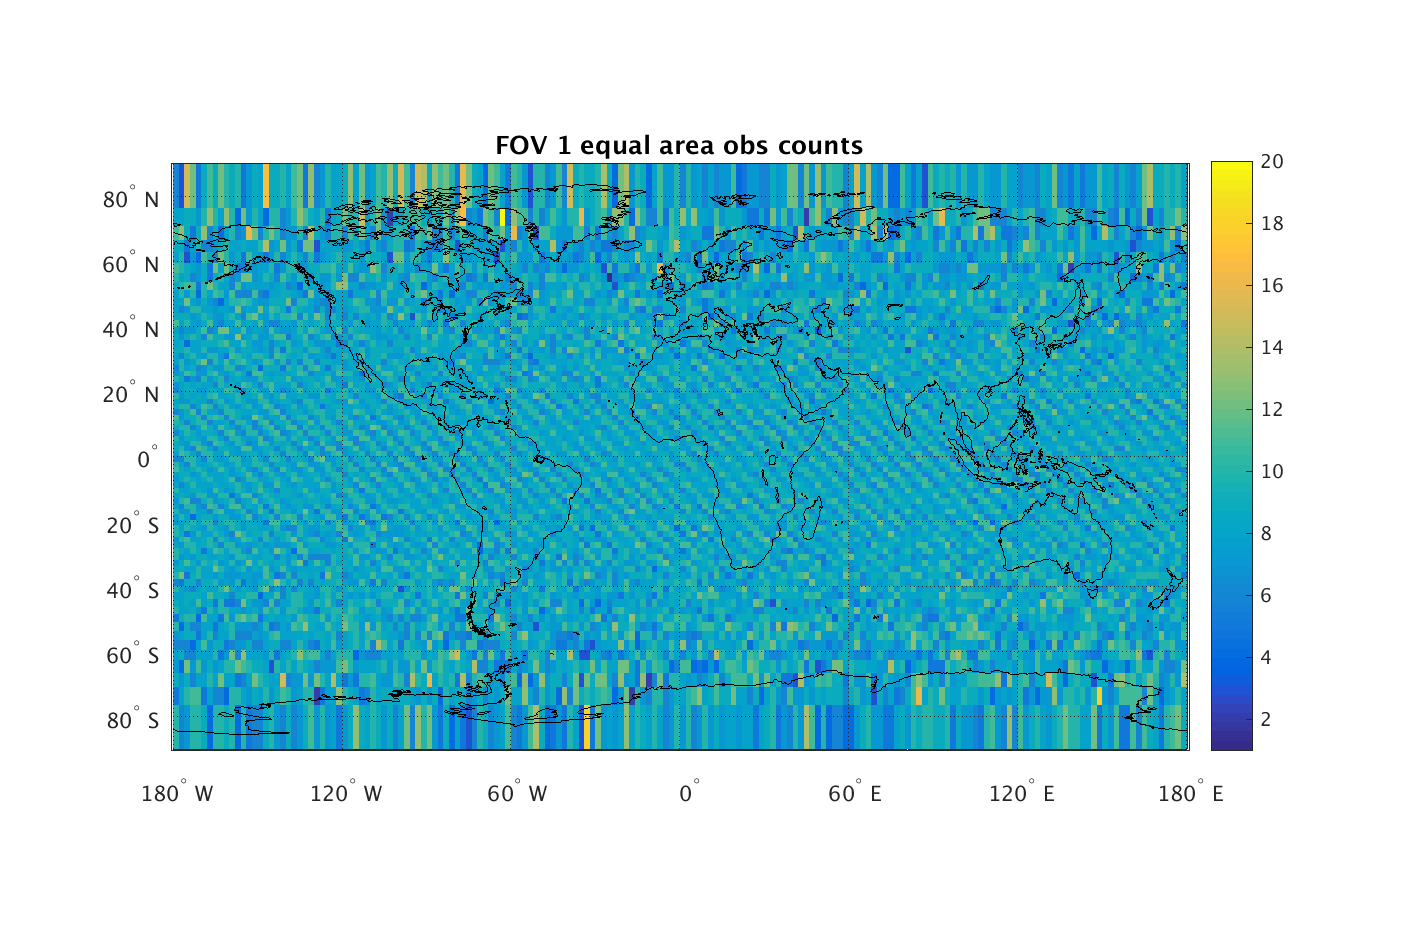
\includegraphics[scale=0.5]{slackfigs/FOV_1_72_bin_desc_counts.png}
\end{center}
\end{frame} % slack/combined sensors 14 July 2017
%----------- slide --------------------------------------------------%
\begin{frame}
\frametitle{FOV 9 minus FOV 1 72 band raw obs diff, descending}
\begin{center}
  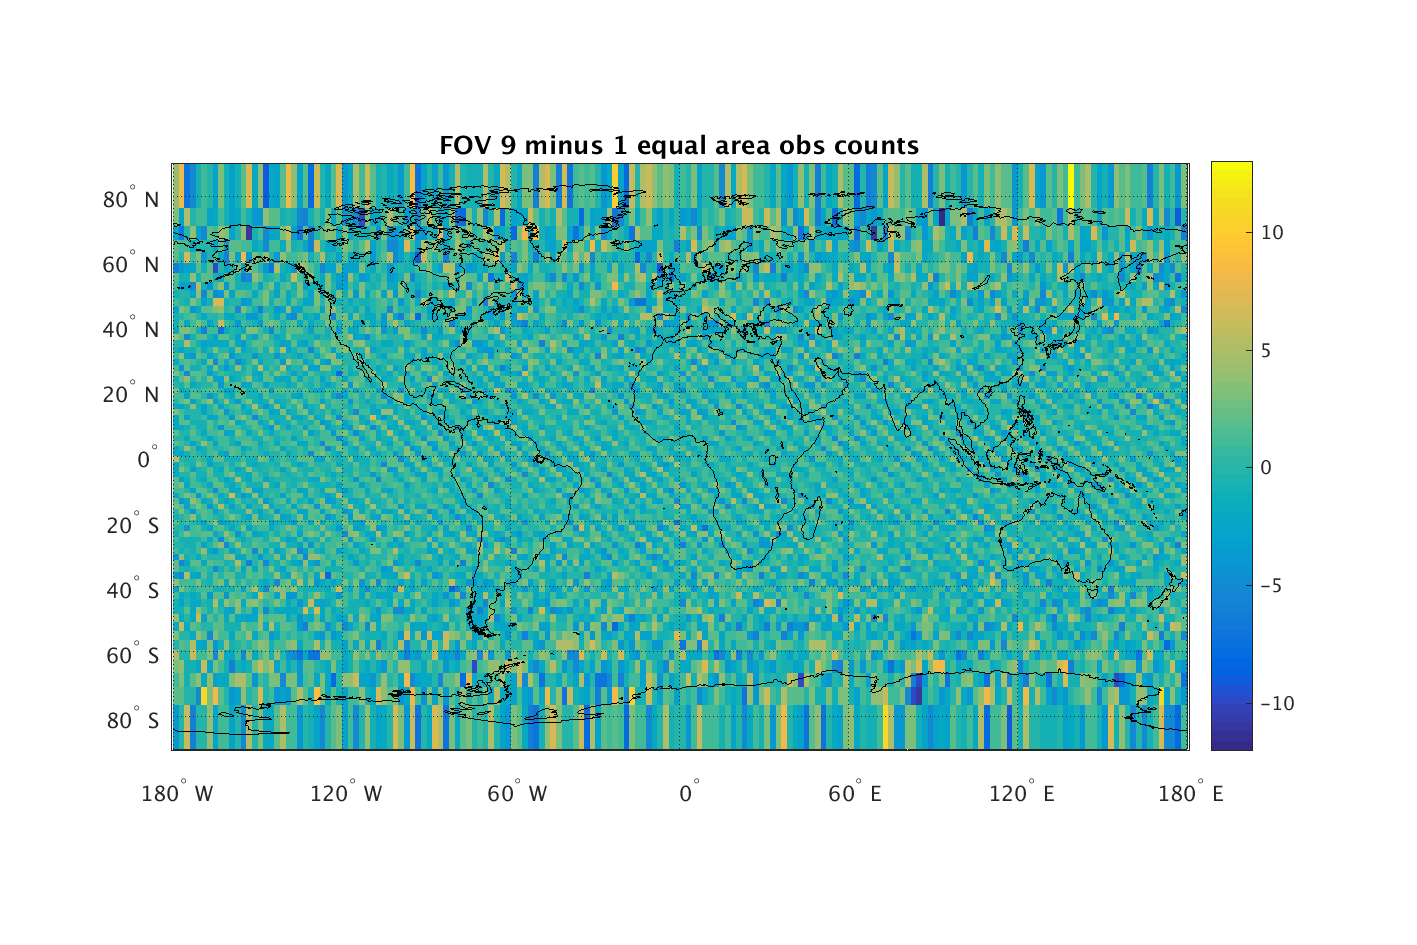
\includegraphics[scale=0.5]{slackfigs/FOV_9_minus_1_72_bin_desc.png}
\end{center}
\end{frame} % slack/combined sensors 14 July 2017
%----------- slide --------------------------------------------------%
\begin{frame}
\frametitle{CrIS FOV comparisons}

\begin{itemize}

  \item in the remaining tests we look at double differences for
    different time spans.  The single differences are FOV 9 minus
    FOV 1, as above 

  \item the first double difference has the second single difference
    shifted by 7 days

  \item the second double difference has the second single difference
    shifted by 16 days, a complete orbital cycle

  \item in theory with all subsetting turned off the double
    difference for the 16 day shift should be zero, because the
    orbital cycle repeates

  \item the remaining residual may be due to some mix of varying QC
    and small actual variation in the obs 

\end{itemize}

\end{frame}
%----------- slide --------------------------------------------------%
\begin{frame}
\frametitle{double difference for a 7 day shift, no subsetting}
\begin{center}
  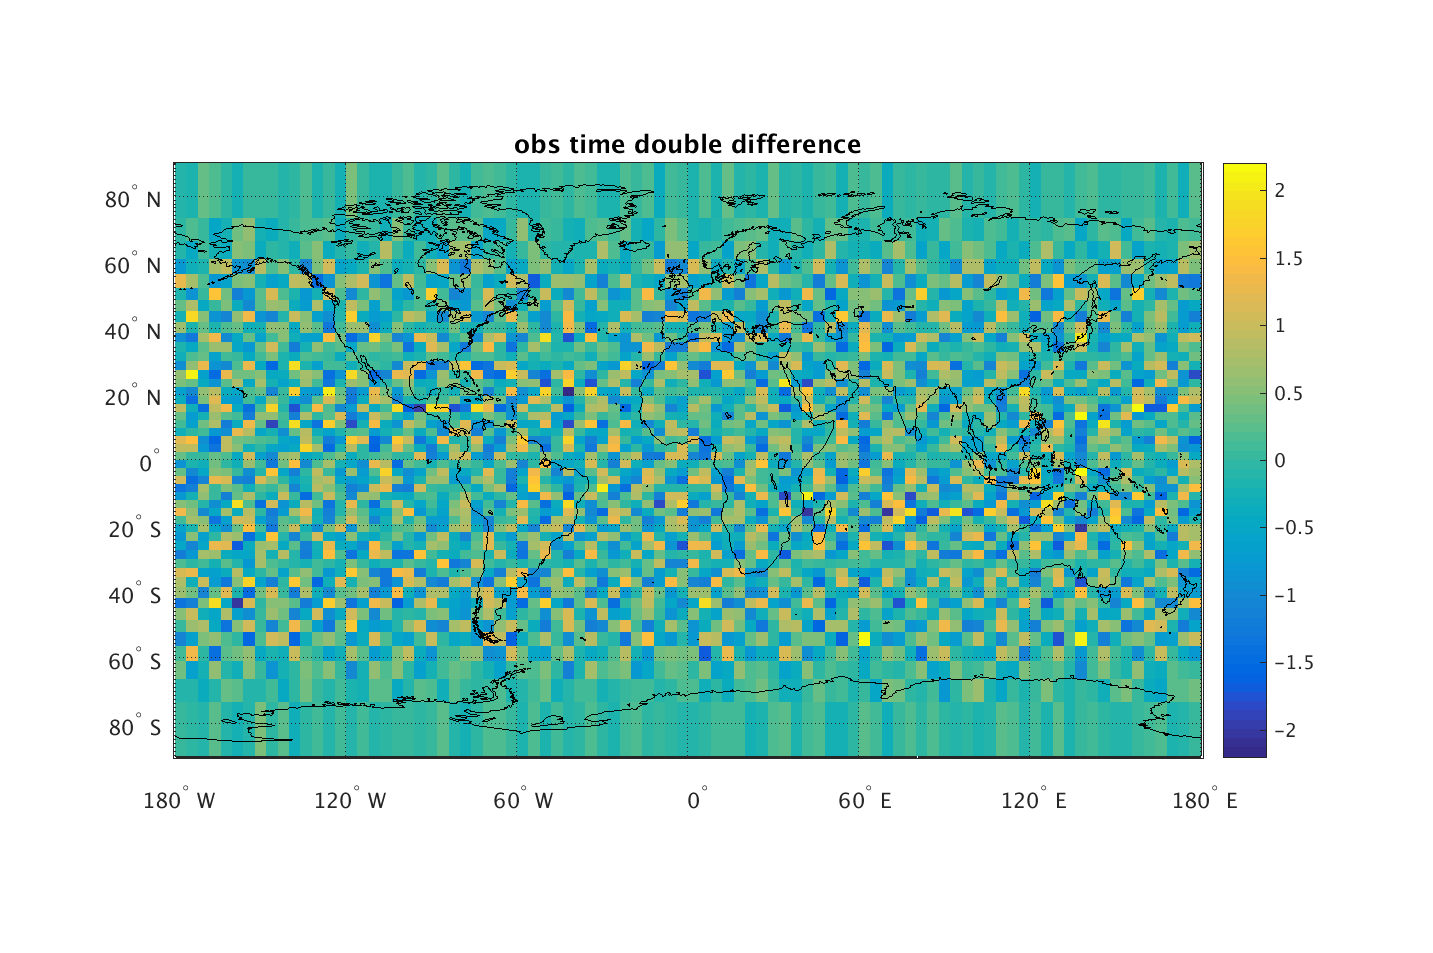
\includegraphics[scale=0.5]{slackfigs/ddiff_7_day_shift.png}
\end{center}
\end{frame} % slack/combined sensors 15 July 2017
%----------- slide --------------------------------------------------%
\begin{frame}
\frametitle{double difference for a 16 day shift, no subsetting}
\begin{center}
  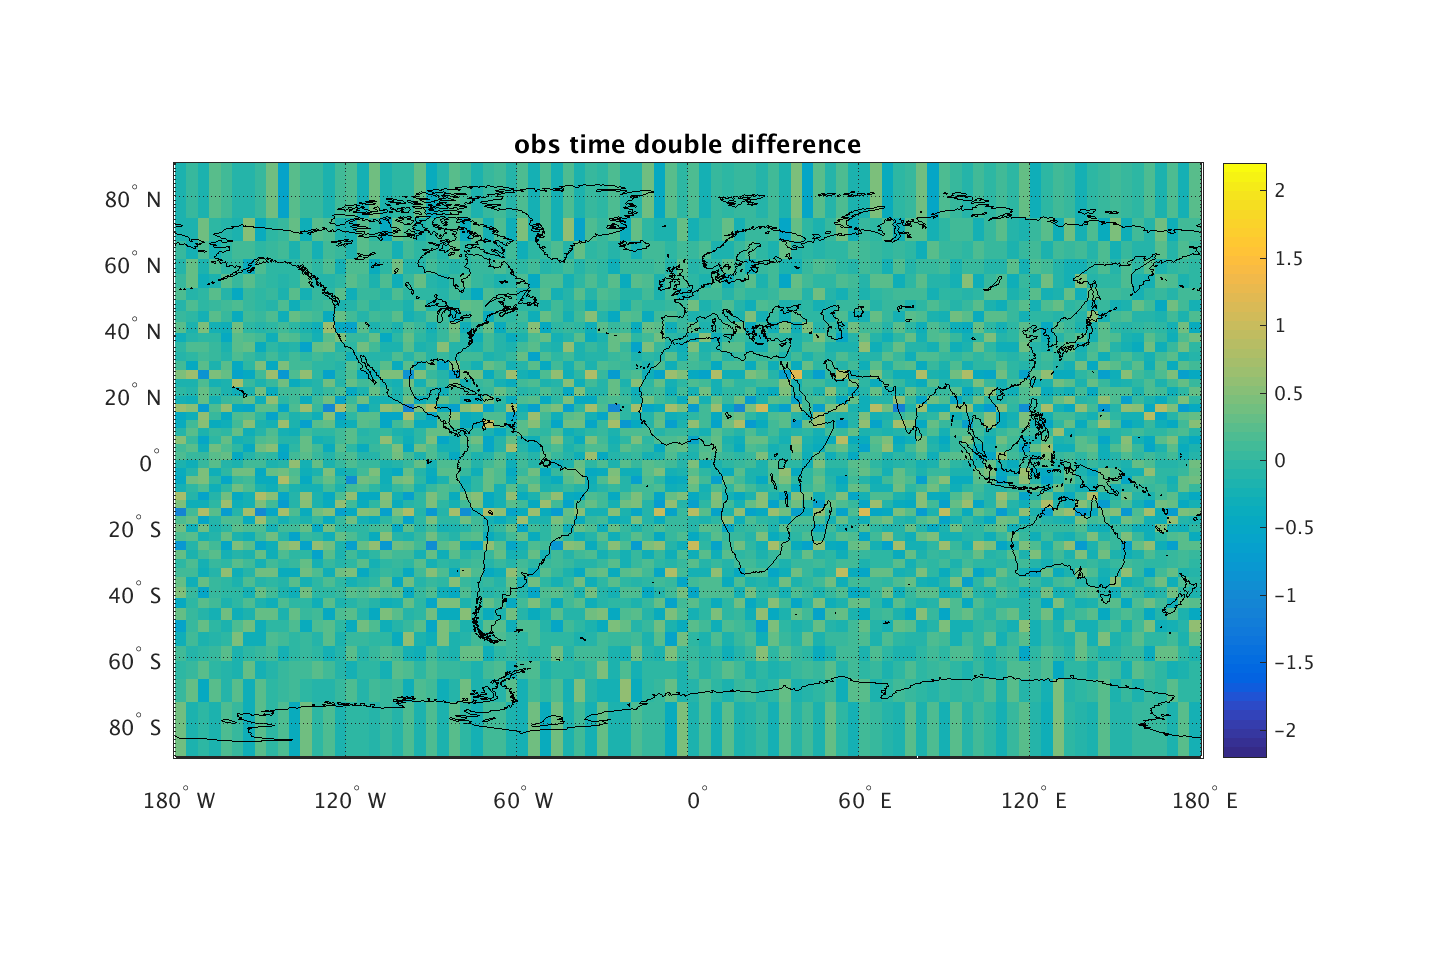
\includegraphics[scale=0.5]{slackfigs/ddiff_16_day_shift.png}
\end{center}
\end{frame} % slack/combined sensors 15 July 2017
%----------- slide --------------------------------------------------%
\begin{frame}
\frametitle{double difference for a 7 day shift, latitude subset}
\begin{center}
  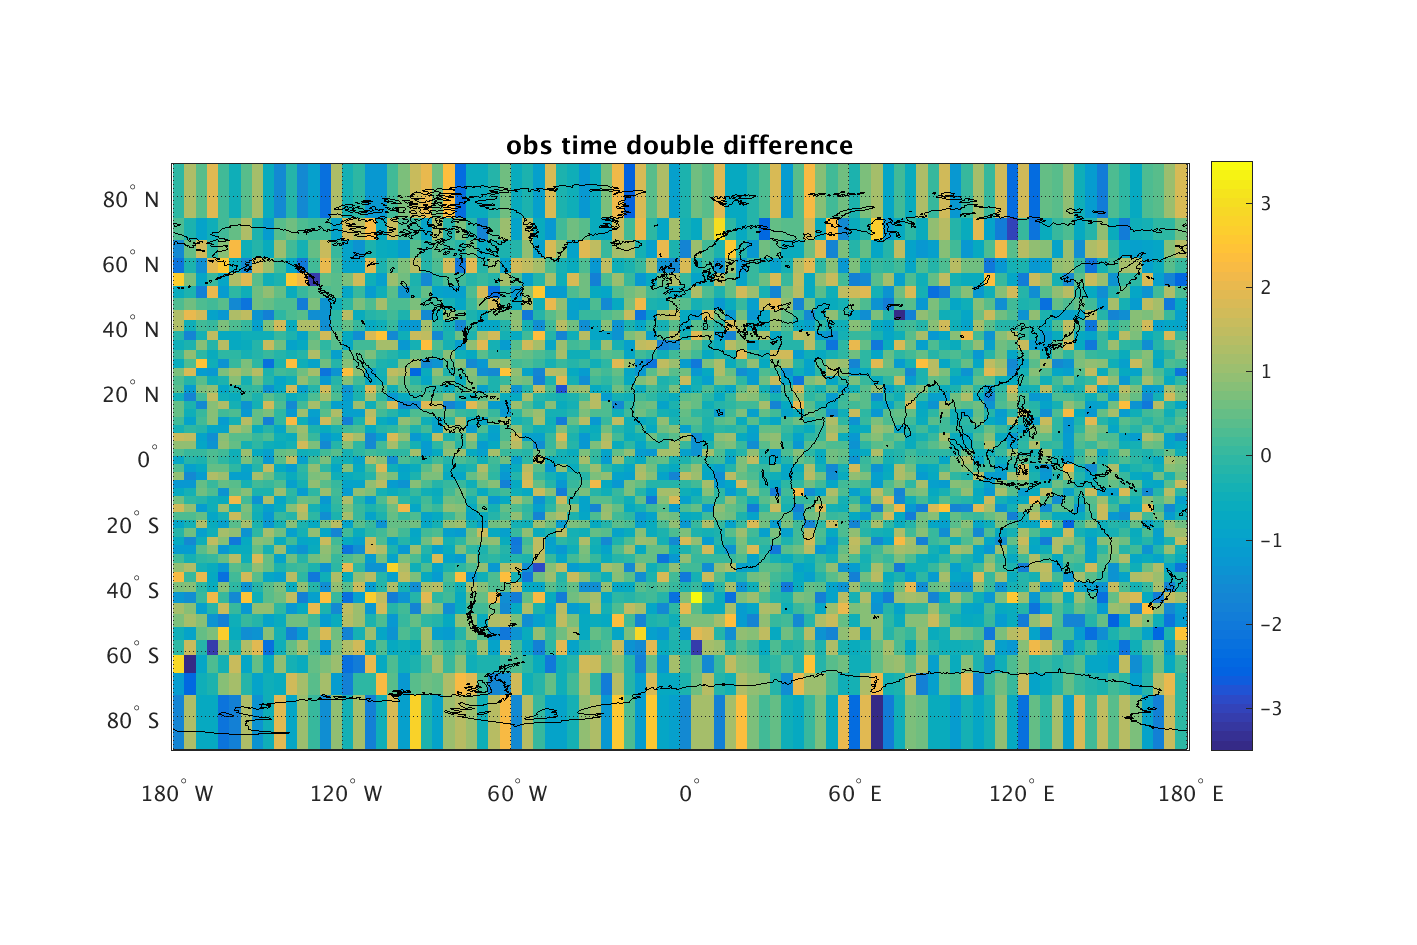
\includegraphics[scale=0.5]{slackfigs/ddiff_7_day_shift_latsub.png}
\end{center}
\end{frame} % slack/combined sensors 15 July 2017
%----------- slide --------------------------------------------------%
\begin{frame}
\frametitle{double difference for a 16 day shift, latitude subset}
\begin{center}
  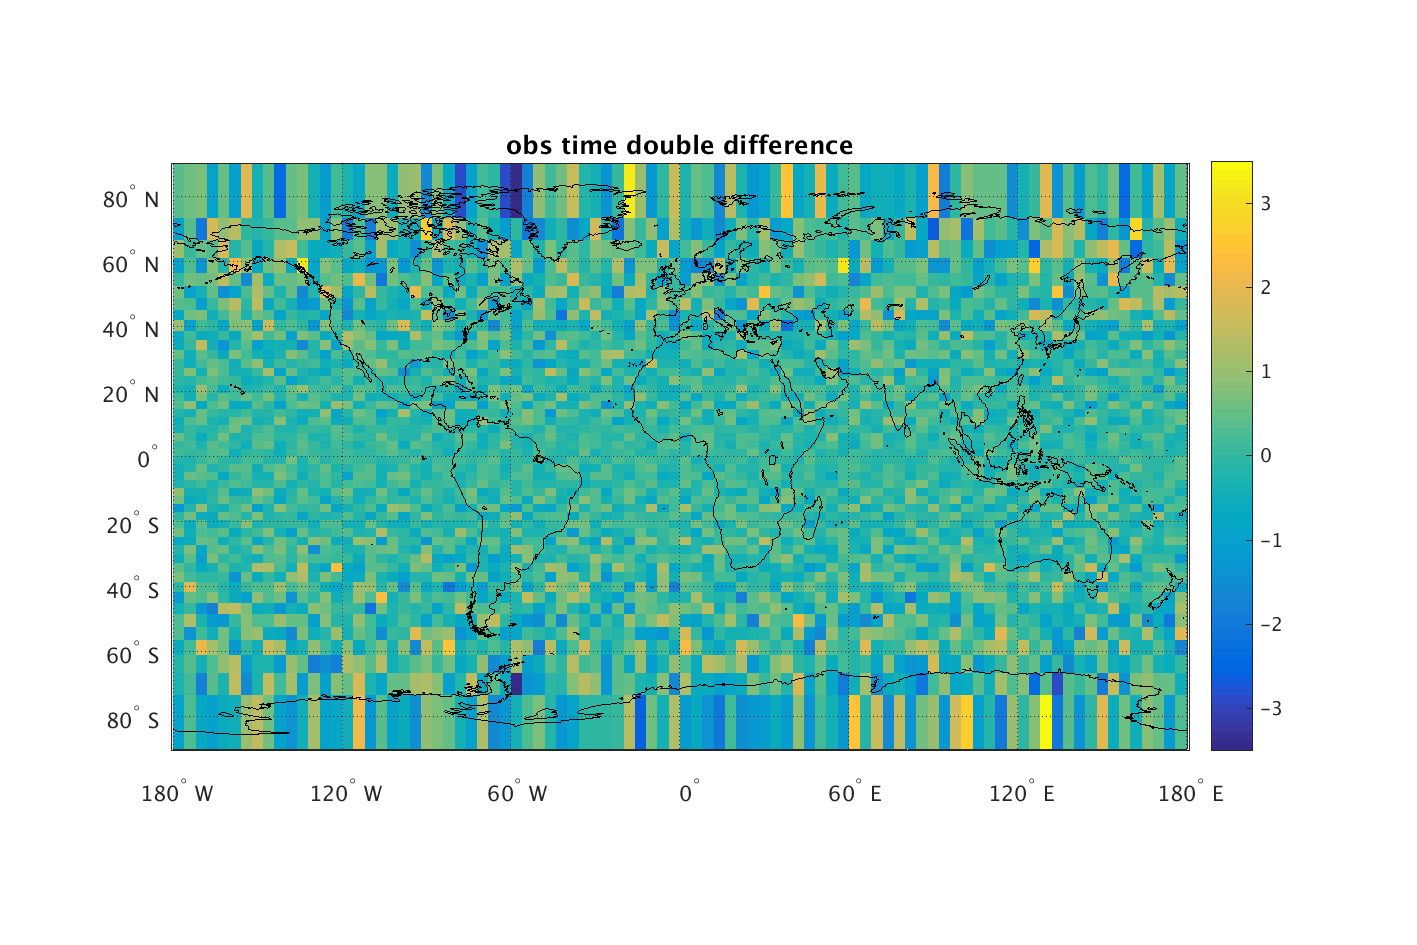
\includegraphics[scale=0.5]{slackfigs/ddiff_16_day_shift_latsub.png}
\end{center}
\end{frame} % slack/combined sensors 15 July 2017
%----------- slide --------------------------------------------------%
\begin{frame}
\frametitle{CrIS FOV comparisons}

\begin{itemize}

  \item adding the latitude weighted subsetting increases the time
    variation and obscures the shifts in the 16 day sampling pattern

  \item the final test is a sort of sanity check on our time
    sampling; we compare FOV 1 alone with no subsetting for 16 and
    32 day periods

  \item our time measure is mean bin time minus mean test time

  \item we would expect this measure to be relatively stable over
    multiples of the 16 day pattern; so for example the means for a
    32 day test would be similar to the means for a 16 day test

  \item as with the double differences this is only partially true

\end{itemize}

\end{frame}
%----------- slide --------------------------------------------------%
\begin{frame}
\frametitle{FOV 1 near-nadir 32 day, no subsetting}
\begin{center}
  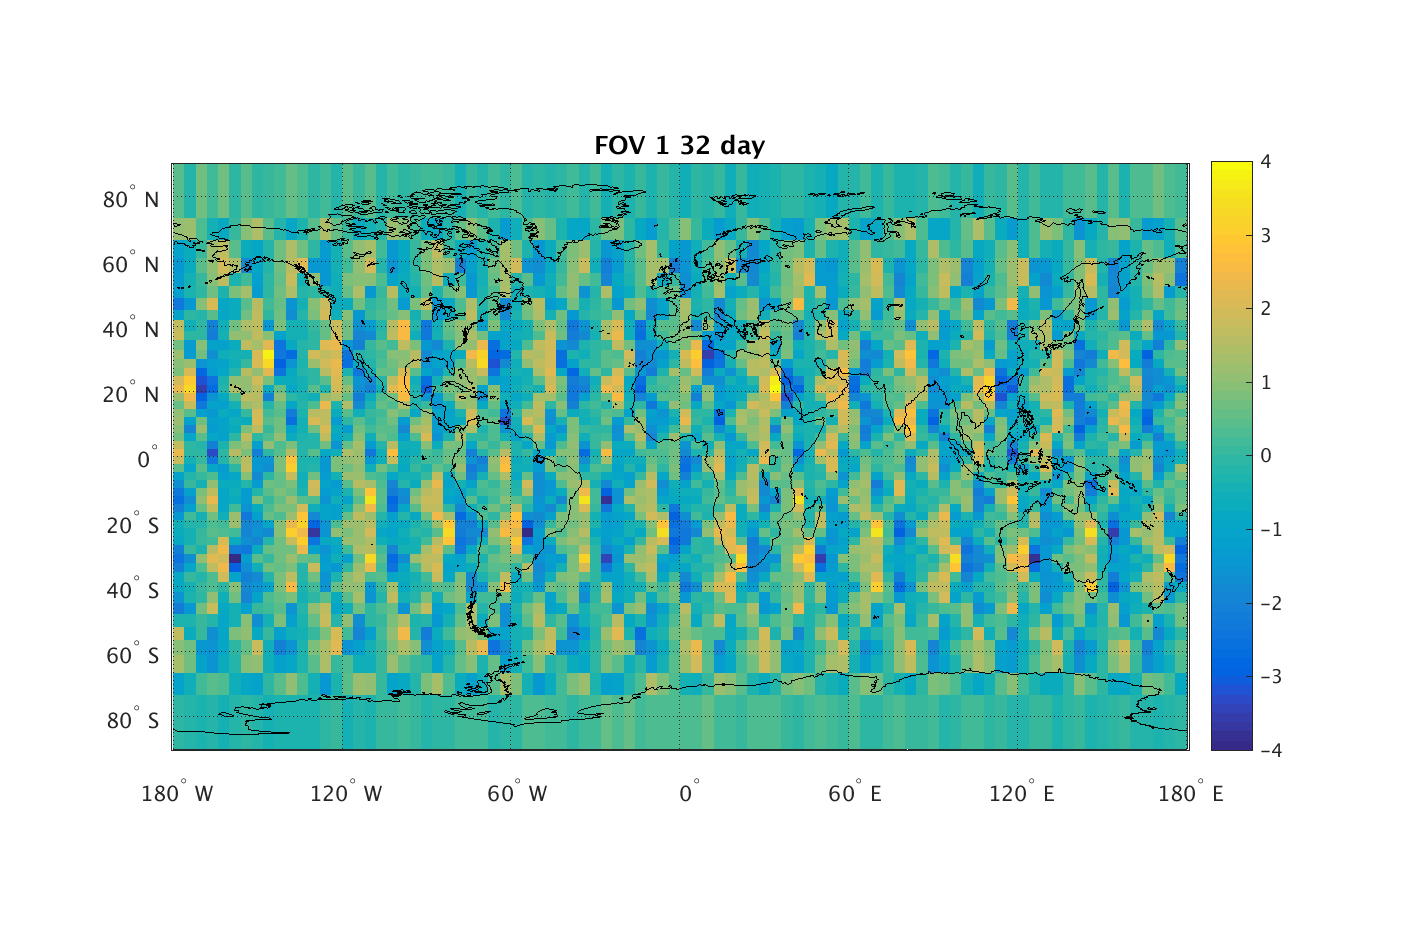
\includegraphics[scale=0.5]{slackfigs/FOV_1_32_day_near_nosub.png}
\end{center}
\end{frame}
%----------- slide --------------------------------------------------%
\begin{frame}
\frametitle{FOV 1 near-nadir 32 day minus 16 day, no subsetting}
\begin{center}
  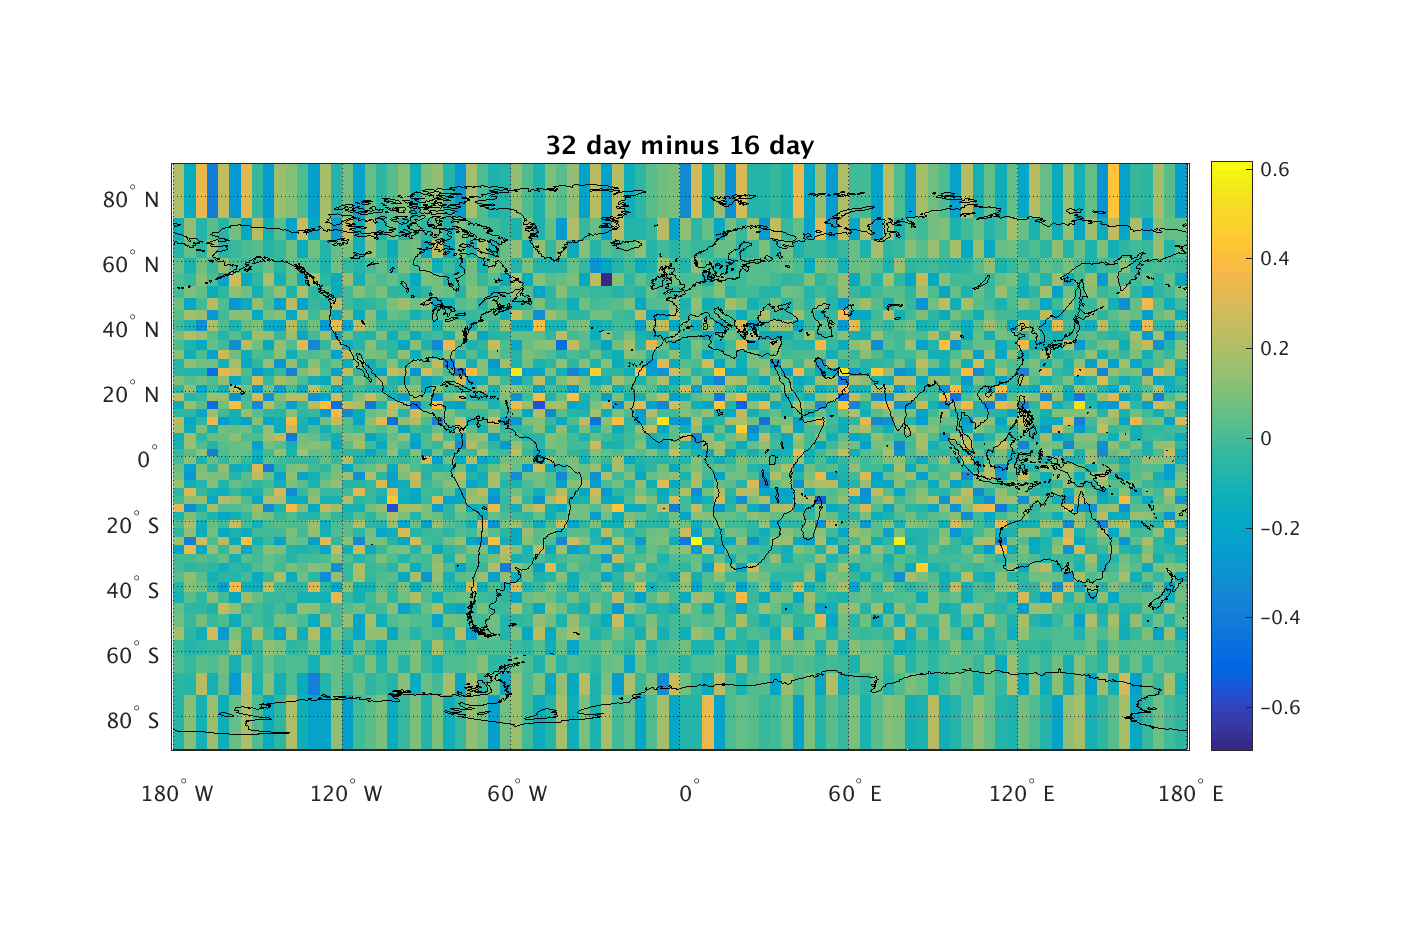
\includegraphics[scale=0.5]{slackfigs/FOV_1_32_minus_16_day_nosub.png}
\end{center}
\end{frame}
% %----------- slide --------------------------------------------------%
% \begin{frame}
% \frametitle{conclusions}
% 
% \begin{itemize}
% 
%   \item with the switch to extended res, we have seen a significant
%     convergence in calibration algorithm performance 
% 
%   \item the {\noaa} ``SA-1 first'' algorithm does slightly better
%     when compared with reference truth convolved with responsivity,
%     while the {\ccast} ``ratio first'' algorithm does slightly
%     better when compared with reference truth convolved with a flat
%     passband
% 
%   \item this may be because responsivity cancels out more completely
%     in the ratio-first method
% 
%   \item because reference truth convolved with a flat passband is a
%     more conventional and non instrument-specific standard, the
%     ccast algorithm, or some similar ratio-first method, may be
%     preferable
% 
% \end{itemize}
% \end{frame}
% %----------- slide --------------------------------------------------%

\end{document}

